%%%%%%%%%%%%%%%%%%%%%%%%%%%%%%%%%%%%%%%%
% Masters/Doctoral Thesis 
% LaTeX Template
% Version 2.5 (27/8/17)
%
% This template was downloaded from:
% http://www.LaTeXTemplates.com
%
% Version 2.x major modifications by:
% Vel (vel@latextemplates.com)
%
% This template is based on a template by:
% Steve Gunn (http://users.ecs.soton.ac.uk/srg/softwaretools/document/templates/)
% Sunil Patel (http://www.sunilpatel.co.uk/thesis-template/)
%
% Template license:
% CC BY-NC-SA 3.0 (http://creativecommons.org/licenses/by-nc-sa/3.0/)
%
%%%%%%%%%%%%%%%%%%%%%%%%%%%%%%%%%%%%%%%%%

%----------------------------------------------------------------------------------------
%	PACKAGES AND OTHER DOCUMENT CONFIGURATIONS
%----------------------------------------------------------------------------------------

\documentclass[
12pt, % The default document font size, options: 10pt, 11pt, 12pt
 % Two side (alternating margins) for binding by default, uncomment to switch to one side
english, % ngerman for German
doublespacing, % Single line spacing, alternatives: onehalfspacing or doublespacing
%draft, % Uncomment to enable draft mode (no pictures, no links, overfull hboxes indicated)
%nolistspacing, % If the document is onehalfspacing or doublespacing, uncomment this to set spacing in lists to single
nolistspacing,
%liststotoc, % Uncomment to add the list of figures/tables/etc to the table of contents
%toctotoc, % Uncomment to add the main table of contents to the table of contents
%parskip, % Uncomment to add space between paragraphs
%nohyperref, % Uncomment to not load the hyperref package
headsepline, % Uncomment to get a line under the header
%chapterinoneline, % Uncomment to place the chapter title next to the number on one line
%consistentlayout, % Uncomment to change the layout of the declaration, abstract and acknowledgements pages to match the default layout
]{MastersDoctoralThesis} % The class file specifying the document structure

\usepackage[utf8]{inputenc} % Required for inputting international characters
\usepackage[T1]{fontenc} % Output font encoding for international characters

\usepackage{mathpazo} % Use the Palatino font by default

\usepackage[backend=bibtex,style=ieee,maxbibnames=3]{biblatex} % Use the bibtex backend with the authoryear citation style (which resembles APA)

\addbibresource{ref.bib} % The filename of the bibliography

\usepackage[autostyle=true]{csquotes} % Required to generate language-dependent quotes in the bibliography

\usepackage{multirow} % Required for some table settings

\usepackage{float} % using % to fix position of figures and tables 

%----------------------------------------------------------------------------------------
%	MARGIN SETTINGS
%----------------------------------------------------------------------------------------

\geometry{
	paper=a4paper, % Change to letterpaper for US letter
	inner=3cm, % Inner margin
	outer=3cm, % Outer margin
	bindingoffset=.5cm, % Binding offset
	top=2cm, % Top margin
	bottom=2cm, % Bottom margin
	%showframe, % Uncomment to show how the type block is set on the page
}

%----------------------------------------------------------------------------------------
%	THESIS INFORMATION
%----------------------------------------------------------------------------------------

\thesistitle{Developments to established dose-finding methodologies for application in trials with complex and innovative designs} % Your thesis title, this is used in the title and abstract, print it elsewhere with \ttitle
\supervisor{Prof. Lucinda \textsc{Billingham}}
% Your supervisor's name, this is used in the title page, print it elsewhere with \supname
\supervisorTWO{Dr. Kristian \textsc{Brock}}
\examiner{} % Your examiner's name, this is not currently used anywhere in the template, print it elsewhere with \examname
\degree{Doctor of Philosophy} % Your degree name, this is used in the title page and abstract, print it elsewhere with \degreename
\author{Amit \textsc{Patel}} % Your name, this is used in the title page and abstract, print it elsewhere with \authorname
\addresses{} % Your address, this is not currently used anywhere in the template, print it elsewhere with \addressname

\subject{Biological Sciences} % Your subject area, this is not currently used anywhere in the template, print it elsewhere with \subjectname
\keywords{} % Keywords for your thesis, this is not currently used anywhere in the template, print it elsewhere with \keywordnames
\university{\href{https://www.birmingham.ac.uk/index.aspx}{University of Birmingham}} % Your university's name and URL, this is used in the title page and abstract, print it elsewhere with \univname
\department{\href{https://www.birmingham.ac.uk/university/colleges/mds/index.aspx}{College of Medical and Dental Sciences}} % Your department's name and URL, this is used in the title page and abstract, print it elsewhere with \deptname
\group{\href{https://www.birmingham.ac.uk/research/cancer-genomics/index.aspx}{Institute of Cancer and Genomic Sciences}} % Your research group's name and URL, this is used in the title page, print it elsewhere with \groupname
\faculty{\href{http://faculty.university.com}{Faculty Name}} % Your faculty's name and URL, this is used in the title page and abstract, print it elsewhere with \facname

\AtBeginDocument{
\hypersetup{pdftitle=\ttitle} % Set the PDF's title to your title
\hypersetup{pdfauthor=\authorname} % Set the PDF's author to your name
\hypersetup{pdfkeywords=\keywordnames} % Set the PDF's keywords to your keywords
}

\begin{document}

\frontmatter % Use roman page numbering style (i, ii, iii, iv...) for the pre-content pages

\pagestyle{plain} % Default to the plain heading style until the thesis style is called for the body content

%----------------------------------------------------------------------------------------
%	TITLE PAGE
%----------------------------------------------------------------------------------------

\begin{titlepage}
\begin{center}

%\vspace*{.06\textheight}
%{\scshape\LARGE \univname\par}\vspace{0.5cm} % University name
\textsc{\Large Doctoral Thesis}\\[0.5cm] % Thesis type

\HRule \\[0.2cm] % Horizontal line
{\Large \bfseries \ttitle\par}\vspace{0.2cm} % Thesis title
\HRule \\[0.5cm] % Horizontal line
 
\begin{minipage}[t]{0.3\textwidth}
\begin{flushleft} \large
\emph{Author:}\\
\href{https://uk.linkedin.com/in/amit-patel-0b718111b}{\authorname} % Author name - remove the \href bracket to remove the link
\end{flushleft}
\end{minipage}
\begin{minipage}[t]{0.5\textwidth}
\begin{flushright} \large
\emph{Supervisor:} \\
\href{https://www.birmingham.ac.uk/staff/profiles/cancer-genomic/billingham-lucinda.aspx}{\supname}\\ % Supervisor name - remove the \href bracket to remove the link  
\href{https://www.kristianbrock.com/}{\supnameTWO}
\end{flushright}
\end{minipage}\\[2.5cm]
 


\large \textit{A thesis submitted in fulfillment of the requirements\\ for the degree of \degreename}\\[2.5cm] % University requirement text



\begin{flushright}
\groupname\\\deptname\\\univname\\\today
\end{flushright}

%\includegraphics{Logo} % University/department logo - uncomment to place it
 
\vfill
\end{center}
\end{titlepage}

%----------------------------------------------------------------------------------------
%	DECLARATION PAGE
%----------------------------------------------------------------------------------------

%\begin{declaration}
%\addchaptertocentry{\authorshipname} % Add the declaration to the table of contents
%\noindent I, \authorname, declare that this thesis titled, \enquote{\ttitle} and the work presented in it are my own. I confirm that:

%\begin{itemize} 
%\item This work was done wholly or mainly while in candidature for a research degree at this University.
%\item Where any part of this thesis has previously been submitted for a degree or any other qualification at this University or any other institution, this has been clearly stated.
%\item Where I have consulted the published work of others, this is always clearly attributed.
%\item Where I have quoted from the work of others, the source is always given. With the exception of such quotations, this thesis is entirely my own work.
%\item I have acknowledged all main sources of help.
%\item Where the thesis is based on work done by myself jointly with others, I have made clear exactly what was done by others and what I have contributed myself.\\
%\end{itemize}
 
%\noindent Signed:\\
%\rule[0.5em]{25em}{0.5pt} % This prints a line for the signature
 
%\noindent Date:\\
%\rule[0.5em]{25em}{0.5pt} % This prints a line to write the date
%\end{declaration}

%\cleardoublepage

%----------------------------------------------------------------------------------------
%	QUOTATION PAGE
%----------------------------------------------------------------------------------------

%\vspace*{0.2\textheight}

%\noindent\enquote{\itshape This is where the fun begins.}\bigbreak

%\hfill Anakin Skywalker

%----------------------------------------------------------------------------------------
%	ABSTRACT PAGE
%----------------------------------------------------------------------------------------

\begin{abstract}
\addchaptertocentry{\abstractname} % Add the abstract to the table of contents
Insert abstract here\ldots
\end{abstract}

%----------------------------------------------------------------------------------------
%	ACKNOWLEDGEMENTS
%----------------------------------------------------------------------------------------

\begin{acknowledgements}
\addchaptertocentry{\acknowledgementname} % Add the acknowledgements to the table of contents
Acknowledge people here \ldots
\end{acknowledgements}

%----------------------------------------------------------------------------------------
%	LIST OF CONTENTS/FIGURES/TABLES PAGES
%----------------------------------------------------------------------------------------

\tableofcontents % Prints the main table of contents

\listoffigures % Prints the list of figures

\listoftables % Prints the list of tables

%----------------------------------------------------------------------------------------
%	ABBREVIATIONS
%----------------------------------------------------------------------------------------

%\begin{abbreviations}{ll} % Include a list of abbreviations (a table of two columns)

%\textbf{LAH} & \textbf{L}ist \textbf{A}bbreviations \textbf{H}ere\\
%\textbf{WSF} & \textbf{W}hat (it) \textbf{S}tands \textbf{F}or\\

%\end{abbreviations}

%----------------------------------------------------------------------------------------
%	PHYSICAL CONSTANTS/OTHER DEFINITIONS
%----------------------------------------------------------------------------------------

%\begin{constants}{lr@{${}={}$}l} % The list of physical constants is a three column table

% The \SI{}{} command is provided by the siunitx package, see its documentation for instructions on how to use it

%Speed of Light & $c_{0}$ & \SI{2.99792458e8}{\meter\per\second} (exact)\\
%Constant Name & $Symbol$ & $Constant Value$ with units\\

%\end{constants}

%----------------------------------------------------------------------------------------
%	SYMBOLS
%----------------------------------------------------------------------------------------

%\begin{symbols}{lll} % Include a list of Symbols (a three column table)

%$a$ & distance & \si{\meter} \\
%$P$ & power & \si{\watt} (\si{\joule\per\second}) \\
%Symbol & Name & Unit \\

%\addlinespace % Gap to separate the Roman symbols from the Greek

%$\omega$ & angular frequency & \si{\radian} \\

%\end{symbols}

%----------------------------------------------------------------------------------------
%	DEDICATION
%----------------------------------------------------------------------------------------

%\dedicatory{For/Dedicated to/To my\ldots} 

%----------------------------------------------------------------------------------------
%	THESIS CONTENT - CHAPTERS
%----------------------------------------------------------------------------------------

\mainmatter % Begin numeric (1,2,3...) page numbering

\pagestyle{thesis} % Return the page headers back to the "thesis" style

% Include the chapters of the thesis as separate files from the Chapters folder
% Uncomment the lines as you write the chapters

% Chapter 1

\chapter{Chapter Title Here} % Main chapter title

\label{Chapter1} % For referencing the chapter elsewhere, use \ref{Chapter1} 

%----------------------------------------------------------------------------------------

% Define some commands to keep the formatting separated from the content 
\newcommand{\keyword}[1]{\textbf{#1}}
\newcommand{\tabhead}[1]{\textbf{#1}}
\newcommand{\code}[1]{\texttt{#1}}
\newcommand{\file}[1]{\texttt{\bfseries#1}}
\newcommand{\option}[1]{\texttt{\itshape#1}}

%----------------------------------------------------------------------------------------

\section{Welcome and Thank You}
Welcome to this \LaTeX{} Thesis Template, a beautiful and easy to use template for writing a thesis using the \LaTeX{} typesetting system.

If you are writing a thesis (or will be in the future) and its subject is technical or mathematical (though it doesn't have to be), then creating it in \LaTeX{} is highly recommended as a way to make sure you can just get down to the essential writing without having to worry over formatting or wasting time arguing with your word processor.

\LaTeX{} is easily able to professionally typeset documents that run to hundreds or thousands of pages long. With simple mark-up commands, it automatically sets out the table of contents, margins, page headers and footers and keeps the formatting consistent and beautiful. One of its main strengths is the way it can easily typeset mathematics, even \emph{heavy} mathematics. Even if those equations are the most horribly twisted and most difficult mathematical problems that can only be solved on a super-computer, you can at least count on \LaTeX{} to make them look stunning.

%----------------------------------------------------------------------------------------

\section{Learning \LaTeX{}}

\LaTeX{} is not a \textsc{wysiwyg} (What You See is What You Get) program, unlike word processors such as Microsoft Word or Apple's Pages. Instead, a document written for \LaTeX{} is actually a simple, plain text file that contains \emph{no formatting}. You tell \LaTeX{} how you want the formatting in the finished document by writing in simple commands amongst the text, for example, if I want to use \emph{italic text for emphasis}, I write the \verb|\emph{text}| command and put the text I want in italics in between the curly braces. This means that \LaTeX{} is a \enquote{mark-up} language, very much like HTML.

\subsection{A (not so short) Introduction to \LaTeX{}}

If you are new to \LaTeX{}, there is a very good eBook -- freely available online as a PDF file -- called, \enquote{The Not So Short Introduction to \LaTeX{}}. The book's title is typically shortened to just \emph{lshort}. You can download the latest version (as it is occasionally updated) from here:
\url{http://www.ctan.org/tex-archive/info/lshort/english/lshort.pdf}

It is also available in several other languages. Find yours from the list on this page: \url{http://www.ctan.org/tex-archive/info/lshort/}

It is recommended to take a little time out to learn how to use \LaTeX{} by creating several, small `test' documents, or having a close look at several templates on:\\ 
\url{http://www.LaTeXTemplates.com}\\ 
Making the effort now means you're not stuck learning the system when what you \emph{really} need to be doing is writing your thesis.

\subsection{A Short Math Guide for \LaTeX{}}

If you are writing a technical or mathematical thesis, then you may want to read the document by the AMS (American Mathematical Society) called, \enquote{A Short Math Guide for \LaTeX{}}. It can be found online here:
\url{http://www.ams.org/tex/amslatex.html}
under the \enquote{Additional Documentation} section towards the bottom of the page.

\subsection{Common \LaTeX{} Math Symbols}
There are a multitude of mathematical symbols available for \LaTeX{} and it would take a great effort to learn the commands for them all. The most common ones you are likely to use are shown on this page:
\url{http://www.sunilpatel.co.uk/latex-type/latex-math-symbols/}

You can use this page as a reference or crib sheet, the symbols are rendered as large, high quality images so you can quickly find the \LaTeX{} command for the symbol you need.

\subsection{\LaTeX{} on a Mac}
 
The \LaTeX{} distribution is available for many systems including Windows, Linux and Mac OS X. The package for OS X is called MacTeX and it contains all the applications you need -- bundled together and pre-customized -- for a fully working \LaTeX{} environment and work flow.
 
MacTeX includes a custom dedicated \LaTeX{} editor called TeXShop for writing your `\file{.tex}' files and BibDesk: a program to manage your references and create your bibliography section just as easily as managing songs and creating playlists in iTunes.

%----------------------------------------------------------------------------------------

\section{Getting Started with this Template}

If you are familiar with \LaTeX{}, then you should explore the directory structure of the template and then proceed to place your own information into the \emph{THESIS INFORMATION} block of the \file{main.tex} file. You can then modify the rest of this file to your unique specifications based on your degree/university. Section \ref{FillingFile} on page \pageref{FillingFile} will help you do this. Make sure you also read section \ref{ThesisConventions} about thesis conventions to get the most out of this template.

If you are new to \LaTeX{} it is recommended that you carry on reading through the rest of the information in this document.

Before you begin using this template you should ensure that its style complies with the thesis style guidelines imposed by your institution. In most cases this template style and layout will be suitable. If it is not, it may only require a small change to bring the template in line with your institution's recommendations. These modifications will need to be done on the \file{MastersDoctoralThesis.cls} file.

\subsection{About this Template}

This \LaTeX{} Thesis Template is originally based and created around a \LaTeX{} style file created by Steve R.\ Gunn from the University of Southampton (UK), department of Electronics and Computer Science. You can find his original thesis style file at his site, here:
\url{http://www.ecs.soton.ac.uk/~srg/softwaretools/document/templates/}

Steve's \file{ecsthesis.cls} was then taken by Sunil Patel who modified it by creating a skeleton framework and folder structure to place the thesis files in. The resulting template can be found on Sunil's site here:
\url{http://www.sunilpatel.co.uk/thesis-template}

Sunil's template was made available through \url{http://www.LaTeXTemplates.com} where it was modified many times based on user requests and questions. Version 2.0 and onwards of this template represents a major modification to Sunil's template and is, in fact, hardly recognisable. The work to make version 2.0 possible was carried out by \href{mailto:vel@latextemplates.com}{Vel} and Johannes Böttcher.

%----------------------------------------------------------------------------------------

\section{What this Template Includes}

\subsection{Folders}

This template comes as a single zip file that expands out to several files and folders. The folder names are mostly self-explanatory:

\keyword{Appendices} -- this is the folder where you put the appendices. Each appendix should go into its own separate \file{.tex} file. An example and template are included in the directory.

\keyword{Chapters} -- this is the folder where you put the thesis chapters. A thesis usually has about six chapters, though there is no hard rule on this. Each chapter should go in its own separate \file{.tex} file and they can be split as:
\begin{itemize}
\item Chapter 1: Introduction to the thesis topic
\item Chapter 2: Background information and theory
\item Chapter 3: (Laboratory) experimental setup
\item Chapter 4: Details of experiment 1
\item Chapter 5: Details of experiment 2
\item Chapter 6: Discussion of the experimental results
\item Chapter 7: Conclusion and future directions
\end{itemize}
This chapter layout is specialised for the experimental sciences, your discipline may be different.

\keyword{Figures} -- this folder contains all figures for the thesis. These are the final images that will go into the thesis document.

\subsection{Files}

Included are also several files, most of them are plain text and you can see their contents in a text editor. After initial compilation, you will see that more auxiliary files are created by \LaTeX{} or BibTeX and which you don't need to delete or worry about:

\keyword{example.bib} -- this is an important file that contains all the bibliographic information and references that you will be citing in the thesis for use with BibTeX. You can write it manually, but there are reference manager programs available that will create and manage it for you. Bibliographies in \LaTeX{} are a large subject and you may need to read about BibTeX before starting with this. Many modern reference managers will allow you to export your references in BibTeX format which greatly eases the amount of work you have to do.

\keyword{MastersDoctoralThesis.cls} -- this is an important file. It is the class file that tells \LaTeX{} how to format the thesis. 

\keyword{main.pdf} -- this is your beautifully typeset thesis (in the PDF file format) created by \LaTeX{}. It is supplied in the PDF with the template and after you compile the template you should get an identical version.

\keyword{main.tex} -- this is an important file. This is the file that you tell \LaTeX{} to compile to produce your thesis as a PDF file. It contains the framework and constructs that tell \LaTeX{} how to layout the thesis. It is heavily commented so you can read exactly what each line of code does and why it is there. After you put your own information into the \emph{THESIS INFORMATION} block -- you have now started your thesis!

Files that are \emph{not} included, but are created by \LaTeX{} as auxiliary files include:

\keyword{main.aux} -- this is an auxiliary file generated by \LaTeX{}, if it is deleted \LaTeX{} simply regenerates it when you run the main \file{.tex} file.

\keyword{main.bbl} -- this is an auxiliary file generated by BibTeX, if it is deleted, BibTeX simply regenerates it when you run the \file{main.aux} file. Whereas the \file{.bib} file contains all the references you have, this \file{.bbl} file contains the references you have actually cited in the thesis and is used to build the bibliography section of the thesis.

\keyword{main.blg} -- this is an auxiliary file generated by BibTeX, if it is deleted BibTeX simply regenerates it when you run the main \file{.aux} file.

\keyword{main.lof} -- this is an auxiliary file generated by \LaTeX{}, if it is deleted \LaTeX{} simply regenerates it when you run the main \file{.tex} file. It tells \LaTeX{} how to build the \emph{List of Figures} section.

\keyword{main.log} -- this is an auxiliary file generated by \LaTeX{}, if it is deleted \LaTeX{} simply regenerates it when you run the main \file{.tex} file. It contains messages from \LaTeX{}, if you receive errors and warnings from \LaTeX{}, they will be in this \file{.log} file.

\keyword{main.lot} -- this is an auxiliary file generated by \LaTeX{}, if it is deleted \LaTeX{} simply regenerates it when you run the main \file{.tex} file. It tells \LaTeX{} how to build the \emph{List of Tables} section.

\keyword{main.out} -- this is an auxiliary file generated by \LaTeX{}, if it is deleted \LaTeX{} simply regenerates it when you run the main \file{.tex} file.

So from this long list, only the files with the \file{.bib}, \file{.cls} and \file{.tex} extensions are the most important ones. The other auxiliary files can be ignored or deleted as \LaTeX{} and BibTeX will regenerate them.

%----------------------------------------------------------------------------------------

\section{Filling in Your Information in the \file{main.tex} File}\label{FillingFile}

You will need to personalise the thesis template and make it your own by filling in your own information. This is done by editing the \file{main.tex} file in a text editor or your favourite LaTeX environment.

Open the file and scroll down to the third large block titled \emph{THESIS INFORMATION} where you can see the entries for \emph{University Name}, \emph{Department Name}, etc \ldots

Fill out the information about yourself, your group and institution. You can also insert web links, if you do, make sure you use the full URL, including the \code{http://} for this. If you don't want these to be linked, simply remove the \verb|\href{url}{name}| and only leave the name.

When you have done this, save the file and recompile \code{main.tex}. All the information you filled in should now be in the PDF, complete with web links. You can now begin your thesis proper!

%----------------------------------------------------------------------------------------

\section{The \code{main.tex} File Explained}

The \file{main.tex} file contains the structure of the thesis. There are plenty of written comments that explain what pages, sections and formatting the \LaTeX{} code is creating. Each major document element is divided into commented blocks with titles in all capitals to make it obvious what the following bit of code is doing. Initially there seems to be a lot of \LaTeX{} code, but this is all formatting, and it has all been taken care of so you don't have to do it.

Begin by checking that your information on the title page is correct. For the thesis declaration, your institution may insist on something different than the text given. If this is the case, just replace what you see with what is required in the \emph{DECLARATION PAGE} block.

Then comes a page which contains a funny quote. You can put your own, or quote your favourite scientist, author, person, and so on. Make sure to put the name of the person who you took the quote from.

Following this is the abstract page which summarises your work in a condensed way and can almost be used as a standalone document to describe what you have done. The text you write will cause the heading to move up so don't worry about running out of space.

Next come the acknowledgements. On this page, write about all the people who you wish to thank (not forgetting parents, partners and your advisor/supervisor).

The contents pages, list of figures and tables are all taken care of for you and do not need to be manually created or edited. The next set of pages are more likely to be optional and can be deleted since they are for a more technical thesis: insert a list of abbreviations you have used in the thesis, then a list of the physical constants and numbers you refer to and finally, a list of mathematical symbols used in any formulae. Making the effort to fill these tables means the reader has a one-stop place to refer to instead of searching the internet and references to try and find out what you meant by certain abbreviations or symbols.

The list of symbols is split into the Roman and Greek alphabets. Whereas the abbreviations and symbols ought to be listed in alphabetical order (and this is \emph{not} done automatically for you) the list of physical constants should be grouped into similar themes.

The next page contains a one line dedication. Who will you dedicate your thesis to?

Finally, there is the block where the chapters are included. Uncomment the lines (delete the \code{\%} character) as you write the chapters. Each chapter should be written in its own file and put into the \emph{Chapters} folder and named \file{Chapter1}, \file{Chapter2}, etc\ldots Similarly for the appendices, uncomment the lines as you need them. Each appendix should go into its own file and placed in the \emph{Appendices} folder.

After the preamble, chapters and appendices finally comes the bibliography. The bibliography style (called \option{authoryear}) is used for the bibliography and is a fully featured style that will even include links to where the referenced paper can be found online. Do not underestimate how grateful your reader will be to find that a reference to a paper is just a click away. Of course, this relies on you putting the URL information into the BibTeX file in the first place.

%----------------------------------------------------------------------------------------

\section{Thesis Features and Conventions}\label{ThesisConventions}

To get the best out of this template, there are a few conventions that you may want to follow.

One of the most important (and most difficult) things to keep track of in such a long document as a thesis is consistency. Using certain conventions and ways of doing things (such as using a Todo list) makes the job easier. Of course, all of these are optional and you can adopt your own method.

\subsection{Printing Format}

This thesis template is designed for double sided printing (i.e. content on the front and back of pages) as most theses are printed and bound this way. Switching to one sided printing is as simple as uncommenting the \option{oneside} option of the \code{documentclass} command at the top of the \file{main.tex} file. You may then wish to adjust the margins to suit specifications from your institution.

The headers for the pages contain the page number on the outer side (so it is easy to flick through to the page you want) and the chapter name on the inner side.

The text is set to 11 point by default with single line spacing, again, you can tune the text size and spacing should you want or need to using the options at the very start of \file{main.tex}. The spacing can be changed similarly by replacing the \option{singlespacing} with \option{onehalfspacing} or \option{doublespacing}.

\subsection{Using US Letter Paper}

The paper size used in the template is A4, which is the standard size in Europe. If you are using this thesis template elsewhere and particularly in the United States, then you may have to change the A4 paper size to the US Letter size. This can be done in the margins settings section in \file{main.tex}.

Due to the differences in the paper size, the resulting margins may be different to what you like or require (as it is common for institutions to dictate certain margin sizes). If this is the case, then the margin sizes can be tweaked by modifying the values in the same block as where you set the paper size. Now your document should be set up for US Letter paper size with suitable margins.

\subsection{References}

The \code{biblatex} package is used to format the bibliography and inserts references such as this one \parencite{Reference1}. The options used in the \file{main.tex} file mean that the in-text citations of references are formatted with the author(s) listed with the date of the publication. Multiple references are separated by semicolons (e.g. \parencite{Reference2, Reference1}) and references with more than three authors only show the first author with \emph{et al.} indicating there are more authors (e.g. \parencite{Reference3}). This is done automatically for you. To see how you use references, have a look at the \file{Chapter1.tex} source file. Many reference managers allow you to simply drag the reference into the document as you type.

Scientific references should come \emph{before} the punctuation mark if there is one (such as a comma or period). The same goes for footnotes\footnote{Such as this footnote, here down at the bottom of the page.}. You can change this but the most important thing is to keep the convention consistent throughout the thesis. Footnotes themselves should be full, descriptive sentences (beginning with a capital letter and ending with a full stop). The APA6 states: \enquote{Footnote numbers should be superscripted, [...], following any punctuation mark except a dash.} The Chicago manual of style states: \enquote{A note number should be placed at the end of a sentence or clause. The number follows any punctuation mark except the dash, which it precedes. It follows a closing parenthesis.}

The bibliography is typeset with references listed in alphabetical order by the first author's last name. This is similar to the APA referencing style. To see how \LaTeX{} typesets the bibliography, have a look at the very end of this document (or just click on the reference number links in in-text citations).

\subsubsection{A Note on bibtex}

The bibtex backend used in the template by default does not correctly handle unicode character encoding (i.e. "international" characters). You may see a warning about this in the compilation log and, if your references contain unicode characters, they may not show up correctly or at all. The solution to this is to use the biber backend instead of the outdated bibtex backend. This is done by finding this in \file{main.tex}: \option{backend=bibtex} and changing it to \option{backend=biber}. You will then need to delete all auxiliary BibTeX files and navigate to the template directory in your terminal (command prompt). Once there, simply type \code{biber main} and biber will compile your bibliography. You can then compile \file{main.tex} as normal and your bibliography will be updated. An alternative is to set up your LaTeX editor to compile with biber instead of bibtex, see \href{http://tex.stackexchange.com/questions/154751/biblatex-with-biber-configuring-my-editor-to-avoid-undefined-citations/}{here} for how to do this for various editors.

\subsection{Tables}

Tables are an important way of displaying your results, below is an example table which was generated with this code:

{\small
\begin{verbatim}
\begin{table}
\caption{The effects of treatments X and Y on the four groups studied.}
\label{tab:treatments}
\centering
\begin{tabular}{l l l}
\toprule
\tabhead{Groups} & \tabhead{Treatment X} & \tabhead{Treatment Y} \\
\midrule
1 & 0.2 & 0.8\\
2 & 0.17 & 0.7\\
3 & 0.24 & 0.75\\
4 & 0.68 & 0.3\\
\bottomrule\\
\end{tabular}
\end{table}
\end{verbatim}
}

\begin{table}
\caption{The effects of treatments X and Y on the four groups studied.}
\label{tab:treatments}
\centering
\begin{tabular}{l l l}
\toprule
\tabhead{Groups} & \tabhead{Treatment X} & \tabhead{Treatment Y} \\
\midrule
1 & 0.2 & 0.8\\
2 & 0.17 & 0.7\\
3 & 0.24 & 0.75\\
4 & 0.68 & 0.3\\
\bottomrule\\
\end{tabular}
\end{table}

You can reference tables with \verb|\ref{<label>}| where the label is defined within the table environment. See \file{Chapter1.tex} for an example of the label and citation (e.g. Table~\ref{tab:treatments}).

\subsection{Figures}

There will hopefully be many figures in your thesis (that should be placed in the \emph{Figures} folder). The way to insert figures into your thesis is to use a code template like this:
\begin{verbatim}
\begin{figure}
\centering

\includegraphics{Figures/Electron}
\decoRule
\caption[An Electron]{An electron (artist's impression).}
\label{fig:Electron}
\end{figure}
\end{verbatim}
Also look in the source file. Putting this code into the source file produces the picture of the electron that you can see in the figure below.

\begin{figure}[th]
\centering

\includegraphics{Figures/Electron}
\decoRule
\caption[An Electron]{An electron (artist's impression).}
\label{fig:Electron}
\end{figure}

Sometimes figures don't always appear where you write them in the source. The placement depends on how much space there is on the page for the figure. Sometimes there is not enough room to fit a figure directly where it should go (in relation to the text) and so \LaTeX{} puts it at the top of the next page. Positioning figures is the job of \LaTeX{} and so you should only worry about making them look good!

Figures usually should have captions just in case you need to refer to them (such as in Figure~\ref{fig:Electron}). The \verb|\caption| command contains two parts, the first part, inside the square brackets is the title that will appear in the \emph{List of Figures}, and so should be short. The second part in the curly brackets should contain the longer and more descriptive caption text.

The \verb|\decoRule| command is optional and simply puts an aesthetic horizontal line below the image. If you do this for one image, do it for all of them.

\LaTeX{} is capable of using images in pdf, jpg and png format.

\subsection{Typesetting mathematics}

If your thesis is going to contain heavy mathematical content, be sure that \LaTeX{} will make it look beautiful, even though it won't be able to solve the equations for you.

The \enquote{Not So Short Introduction to \LaTeX} (available on \href{http://www.ctan.org/tex-archive/info/lshort/english/lshort.pdf}{CTAN}) should tell you everything you need to know for most cases of typesetting mathematics. If you need more information, a much more thorough mathematical guide is available from the AMS called, \enquote{A Short Math Guide to \LaTeX} and can be downloaded from:
\url{ftp://ftp.ams.org/pub/tex/doc/amsmath/short-math-guide.pdf}

There are many different \LaTeX{} symbols to remember, luckily you can find the most common symbols in \href{http://ctan.org/pkg/comprehensive}{The Comprehensive \LaTeX~Symbol List}.

You can write an equation, which is automatically given an equation number by \LaTeX{} like this:
\begin{verbatim}
\begin{equation}
E = mc^{2}
\label{eqn:Einstein}
\end{equation}
\end{verbatim}

This will produce Einstein's famous energy-matter equivalence equation:
\begin{equation}
E = mc^{2}
\label{eqn:Einstein}
\end{equation}

All equations you write (which are not in the middle of paragraph text) are automatically given equation numbers by \LaTeX{}. If you don't want a particular equation numbered, use the unnumbered form:
\begin{verbatim}
\[ a^{2}=4 \]
\end{verbatim}

%----------------------------------------------------------------------------------------

\section{Sectioning and Subsectioning}

You should break your thesis up into nice, bite-sized sections and subsections. \LaTeX{} automatically builds a table of Contents by looking at all the \verb|\chapter{}|, \verb|\section{}|  and \verb|\subsection{}| commands you write in the source.

The Table of Contents should only list the sections to three (3) levels. A \verb|chapter{}| is level zero (0). A \verb|\section{}| is level one (1) and so a \verb|\subsection{}| is level two (2). In your thesis it is likely that you will even use a \verb|subsubsection{}|, which is level three (3). The depth to which the Table of Contents is formatted is set within \file{MastersDoctoralThesis.cls}. If you need this changed, you can do it in \file{main.tex}.

%----------------------------------------------------------------------------------------

\section{In Closing}

You have reached the end of this mini-guide. You can now rename or overwrite this pdf file and begin writing your own \file{Chapter1.tex} and the rest of your thesis. The easy work of setting up the structure and framework has been taken care of for you. It's now your job to fill it out!

Good luck and have lots of fun!

\begin{flushright}
Guide written by ---\\
Sunil Patel: \href{http://www.sunilpatel.co.uk}{www.sunilpatel.co.uk}\\
Vel: \href{http://www.LaTeXTemplates.com}{LaTeXTemplates.com}
\end{flushright}

% Chapter Template

\chapter{Implementing the PO-TITE-CRM trial design into ADePT-DDR} % Main chapter title

\label{Chapter2} % For referencing this chapter elsewhere, use \ref{Chapter2}

%----------------------------------------------------------------------------------------
%	SECTION 1
%----------------------------------------------------------------------------------------

\section{Introduction}

Worldwide there are approximately 600,000 new cases of Head and Neck Squamous Cell Carcinoma (HNSCC) each year \cite{stranskyMutationalLandscapeHead2011}. Of which, 12,000 occur in the UK with the most common forms of treatment being surgery, radiotherapy and/or chemotherapy \cite{cancerreaserchukHeadNeckCancers2017}. Radiotherapy is essential for the treatment of cancer. It has been estimated that more than 40\% of patients will receive radiotherapy at some point in their treatment \cite{roundRadiotherapyDemandActivity2013}. However, despite recent advancements in radiation techniques and the use of concomitant chemo radiotherapy, patients with solid tumours such as head and neck cancer have suboptimal cure rates \cite{cancerreaserchukHeadNeckCancers2017,cognettiHeadNeckCancer2008}. For those with advanced HNSCC primary radiotherapy with concurrent chemotherapy is often offered but, it has not been shown to improve survival in patients aged over 70 compared to radiotherapy alone \cite{pignonChemotherapyAddedLocoregional2000}. Therefore, any strategy to improve the efficacy of radiotherapy without increasing toxicity would have a significant impact on patient outcomes. 

DNA damage repair (DDR) inhibition is a potential technique which could be utilised as it potentiates the therapeutic effects of ionising radiation in cancer cells \cite{oconnorTargetingDNADamage2015}. Combining radiotherapy with DDR inhibition could improve clinical outcomes for these patients \cite{chalmersScienceFocusCombining2016}.  

The ADePT-DDR trial is a platform trial which aims to evaluate the safety and efficacy of different DDR agents, or different immunotherapy agents and/or DDR and immunotherapy combinations, together with radiotherapy in patients with HNSCC. The initial component of this trial is a single-arm dose-finding trial investigating the ataxia telangiectasis and Rad3-related (ATR) inhibitor AZD6738 in combination with radiotherapy. ATR inhibitors not only stop DNA repair but impair the mechanism that allows for repairs to take place. Preclinical models have shown this double blocking to be effective in killing cancer cells \cite{meiAtaxiaTelangiectasiaRad3related2019}. 

Traditionally dose-finding trials aim to determine the maximum tolerated dose (MTD) of a treatment based on the cytotoxic assumption that the most toxic dose is the most efficacious. Rule-based or 'up and down' designs achieve this by escalating and de-escalating doses dependent on the observation of severe toxicity due to the drug,  commonly referred to as a dose-limiting toxicity (DLT). In the case of the 3+3 design escalation continues until at least two patients in a cohort of three or six experience a DLT. More explicitly, the MTD is the dose level below the dose at which $\geq$33\% of patients experience a DLT \cite{letourneauDoseEscalationMethods2009}. Model-based designs such as the continual reassessment method (CRM) \cite{oquigleyContinualReassessmentMethod1990} work on the assumption that the probability of toxicity increases monotonically with increases in dose levels. The CRM aims to find the MTD which is a dose with specified target toxicity level. 

Due to the historical use of rule-based designs  \cite{rogatkoTranslationInnovativeDesigns2007, chiuzanDosefindingDesignsTrials2017}, the majority of the terminology used to describe them, and the ambiguity they raise, has been inherited by modern designs such as the CRM. The MTD in the context of a CRM is not the 'maximum' dose patients could tolerate but rather a dose in which there would be an acceptable target probability of a DLT occurring. For example, if the target is set at 25\% the MTD would be the dose at which there is a 25\% probability of experiencing a DLT. Rather than using the term MTD, the dose to be found will be referred to as the target dose (TD\%\%, where the \%'s are replaced by the target probability), i.e. TD25 would be the dose expected to be toxic in 25\% of patients.

The investigation of multiple-agent treatments, where the monotonicity assumption may not hold, is increasing in early phase trials. Finding the TD in combinations of treatments, compared to single-agents,  presents methodological challenges. Each drug individually may obey the monotonicity assumption, however, when combined, the ordering of doses in terms of toxicity may not be fully apparent. An order for a subset of the combined doses could be identified resulting in a partial order. Without a fully understood ordering it is uncertain which dose should be chosen in decisions of escalation and de-escalation and ultimately as the TD. This issue is not exclusively reserved for trials with multiple-agents. The monotonicity assumption may not hold for certain drugs in single-agent studies leading to partial orders of dose toxicity. Monotonicity is a very strong assumption. It requires that probability of toxicity always increases - staying the same is not enough. At high enough doses, this assumption is almost surely violated for all interventions when the event probability reaches its maximum. Thus, even when total ordering is possible, the monotonicity assumption could be violated \cite{brockMoreBetterAnalysis2020}. This can occur in scenarios where multiple parameters of the treatment schedule are altered for each dose level. For example, either dose or treatment duration could be increased and even if patients receive an equal dose it would remain unclear as to if prolonged exposure to a lower dose is more toxic than short exposure to a higher dose, which implies a partial ordering of toxicity probabilities. 

Further methodological challenges revolve around the issue of late-onset toxicities. Typically, early phase trials implement a short window to observe DLTs. This works well in situations where toxicities are likely to occur rapidly after treatment. However, this is not optimal for treatments that could cause late-onset toxicities such as radiotherapy. The aim here would be to incorporate a larger observation window to account for potential late-onset toxicities whilst also minimising the trial duration. 

Cheung and Chappel \cite{cheungSequentialDesignsPhase2000} introduced an extension to the CRM to deal with the issues of treatments that may cause late-onset toxicity. This design referred to as the time-to-event CRM (TITE-CRM), uses a weighted dose-response model to incorporate the time it takes for a DLT to occur in a patient. There have also been published trial designs to deal with the issues that arise from investigating combinations of treatments. Thall et al. \cite{thallDoseFindingTwoAgents2003} proposed an adaptive two-stage Bayesian design which utilises a parametric model of toxicity as a function of two doses. Yin and Yuan \cite{yinBayesianDoseFinding2009} present a Bayesian design that uses a copula regression model to evaluate the joint toxicity probabilities of combined drugs. The continual reassessment method for partial orders (PO-CRM) developed by Wages et al. \cite{wagesContinualReassessmentMethod2011} extends the CRM design by relaxing the assumption of monotonicity and by modelling different potential orders. Figure \ref{fig_adept:example_dose_levels} shows a simple example of partial ordering where the order of two out of the four dose levels are unknown. 

\begin{figure}[h!]
	\centering
	\caption{Example dose levels to illustrate partial ordering.}
	\label{fig_adept:example_dose_levels}
	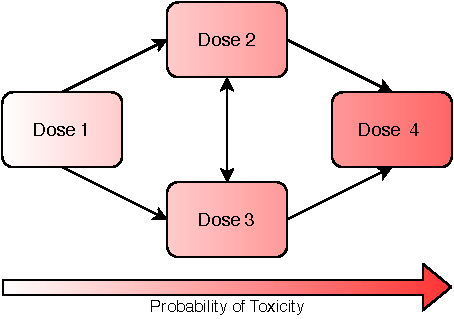
\includegraphics[width=0.75\textwidth]{AdeptDoseExample}
\end{figure}

Wages et al. \cite{wagesContinualReassessmentMethod2011, wagesUsingTimetoeventContinual2013} further developed their work on the PO-CRM to deal with late-onset toxicities by implementing a TITE component. This trial design, referred to as the time-to-event continual reassessment method in the presence of partial orders (PO-TITE-CRM) by the authors, was chosen to be used in ADePT-DDR. A search of PubMed, conducted on the 25th of July 2020, found six articles that had cited the PO-TITE-CRM design by Wages et al. \cite{wagesUsingTimetoeventContinual2013}. Five of these papers were methodological in nature, two of which only include the PO-TITE-CRM design in a brief introduction to current methodology before going on to present new Bayesian trial designs \cite{liuBAYESIANDATAAUGMENTATION2013, wheelerBayesianModelfreeApproach2019}. The other three papers were authored by Wages. The first of which details practical considerations and specifications for the PO-CRM design, the TITE variant is only cited as the source of an example which is being used \cite{wagesSpecificationsContinualReassessment2013}. One paper presents an R package 'pocrm' \cite{wagesPocrmRpackagePhase2013, wagesPocrmDoseFinding2019}. The package is only capable of analysing the PO-CRM design. The TITE variant is only referenced here as it illustrates the issue of partial ordering. The last methodological paper by Wages et al. \cite{wagesPracticalDesignsPhase2016} presents three different methods for phase \RN{1} studies of drug combinations one of which is the PO-CRM however, PO-TITE-CRM is only mentioned as an extension to this design. A key message in this paper is the fact that novel methodologies are constantly emerging but are rarely implemented in practice. 

The last paper is a protocol paper for a phase \RN{1}/\RN{2} study, OLA-TMZ-RTE-01 \cite{lesueurPhaseIIaStudy2019}. The phase \RN{1} component of the study aims to determine the recommended phase \RN{2} dose (RP2D) of olaparib combined with a standard schedule of radiotherapy and temozolomide (TMZ) as first line treatment for patients with unresectable glioblastoma (GBM). The treatment schedule is divided into a radiotherapy and maintenance period. They propose to conduct two sequential dose-escalations of seven different  olaparib dose-levels. Patients in the first escalation will be allocated to a dose level of olaparib for 10 weeks including radiotherapy for six weeks with TMZ given each day during radiotherapy and then for six cycles four weeks post radiotherapy during the maintenance period. They state the MTD1 will be determined using a TITE-CRM. Patients in the second escalation olaparib at the MTD1 during the radiotherapy period along with the same schedule of radiotherapy and TMZ. Those patients will then be allocated to one of the seven dose levels of olaparib during the maintenance period. Again, it is stated that the MTD2 will be determined using TITE-CRM modelling. The RP2D is the MTD1 and MTD2 during the radiotherapy and maintenance period respectively. Even though a combination of treatments is being investigated only olaparib is being escalated and doses for other treatments are fixed for all patients. Furthermore, the dose-levels for olaparib increase consistently in either amount or duration meaning there are no issues of partial ordering which would warrant the use of PO-TITE-CRM. The authors reference the TITE-CRM methodology with two papers. One of them being the paper detailing the PO-TITE-CRM design and the other being a paper by Huang and Kuan \cite{huangTimetoeventContinualReassessment2014} which proposes an adaptive weight function that incorporates cyclical data of treatment into the TITE-CRM. It is unclear as to why the PO-TITE-CRM is cited as its methodology is not mentioned anywhere in methods.       

This is just a brief review of the current literature but it seems that the PO-TITE-CRM has rarely been used or discussed since its inception. 

This chapter provides novel insight into the methodology of PO-TITE-CRM through application in a real-world scenario. Section \ref{section2.2} will detail how the PO-TITE-CRM works. Section \ref{section2.3} discusses the justification for implementing the design into the ADePT-DDR trial and our experiences doing so.  

%----------------------------------------------------------------------------------------
%	SECTION 2
%----------------------------------------------------------------------------------------
\section{The PO-TITE-CRM Design}
\label{section2.2} %first number is the chapter number, second number is section number, third is subsection etc...

Wages et al. \cite{wagesUsingTimetoeventContinual2013} introduced the PO-TITE-CRM design which builds directly upon the PO-CRM design by incorporating a TITE component into the dose toxicity model. The aim of which is to determine the target dose for combinations of drugs where the monotonicity assumption does not hold, in a setting where late-onset toxicities are possible.

\begin{table}[h!]
	\centering
	\caption[Example drug combinations with two agents.]{Example of drug combinations for a trial investigating two agents.}
	\label{tab_adept:ex_drug_combo}
	\begin{tabular}{lcccccc}
		\hline  & \multicolumn{6}{c}{\textbf{Drug combinations}}  \\
		\textbf{Agent} & $d_{1}$ & $d_{2}$ & $d_{3}$ & $d_{4}$ & $d_{5}$ & $d_{6}$ \\ \hline
		A (mg/day) & 0.25 & 0.5 & 1.0 & 0.25 & 0.5 & 1.0         \\
		B (mg/day) & 1.0  & 1.0 & 1.0 & 1.5  & 1.5 & 1.5         \\ \hline
	\end{tabular}
\end{table}

To help understand partial ordering consider an example of an early phase trial investigating the combination of two agents. Drug A which consists of three doses (0.25, 0.5, 1.0 mg/day) and drug B which consists of two doses (1.0, 1.5 mg/day), for a total of six drug combinations $d_{1}$, ..., $d_{6}$ (Table \ref{tab_adept:ex_drug_combo}). For each drug independently we assume they have a monotonic dose-toxicity curve however, the ordering of toxicity probabilities for some of the treatment combinations is unknown. Specifically, we can say $d_{1}$ is less toxic than $d_{2}$ as the dose of drug A increased whilst the dose of drug B stayed the same. This is also the case for $d_{2}$ and $d_{3}$. The order between $d_{4}$ and $d_{5}$ in comparison to $d_{3}$ is not known because the dose of drug A decreases whilst the dose of drug B increases. Assessing all these potential order toxicity relationships leaves five possible orderings. 

\begin{enumerate}
	\centering
	\item $d_{1} \rightarrow d_{2} \rightarrow d_{3} \rightarrow d_{4} \rightarrow d_{5} \rightarrow d_{6}$
	\item $d_{1} \rightarrow d_{2} \rightarrow d_{4} \rightarrow d_{3} \rightarrow d_{5} \rightarrow d_{6}$
	\item $d_{1} \rightarrow d_{2} \rightarrow d_{4} \rightarrow d_{5} \rightarrow d_{3} \rightarrow d_{6}$
	\item $d_{1} \rightarrow d_{4} \rightarrow d_{2} \rightarrow d_{3} \rightarrow d_{5} \rightarrow d_{6}$
	\item $d_{1} \rightarrow d_{4} \rightarrow d_{2} \rightarrow d_{5} \rightarrow d_{3} \rightarrow d_{6}$
\end{enumerate}


Using the notation of Wages et al. \cite{wagesContinualReassessmentMethod2011,wagesUsingTimetoeventContinual2013}, let $M$ denote the number of possible orders and $Y$ be an indicator of a toxicity event. Then for a trial investigating $k$ combinations, $d_{1}$,...,$d_{k}$, the dose for the $j$th patient, $X_{j}$, $j$ = 1,...,$n$ can be thought of as random $x_{j} \in (d_{1}, ..., d_{k})$. For a specific ordering $m$, $m = 1,...,M$ the toxicity probability $R(d_{i})$ is modelled by 
\begin{equation}
R(d_{i}) =  \phi_m(d_i,w,\beta) = w\psi_m(d_i,\beta) \; i = 1, ..., k; \; m = 1, ...,M
\end{equation}
for  a weighted dose response model $\phi_m(d_i,w,\beta)$ where $\beta \in (-\infty, \infty)$. The weight, $w$ as defined by Cheung and Chappel \cite{cheungSequentialDesignsPhase2000}, is a function of the time-to-event of each patient and is incorporated linearly with the dose toxicity model $\psi$ so that $0 \leq w \leq 1$. Each patient is followed for a fixed amount of time $T$. Let $U_j$ represent the time-to-toxicity of patient $j$. Then for $u \leq T$, 
\begin{equation}
	P(U_j \leq u ) = P(U_j \leq u |U_j \leq T)P(U_j \leq T) \equiv w(u;T) \psi_m(d_i,\beta).
\end{equation}
For simplicity we will refer to the weight function $w(u;T)$ as $w$. The weight function will have to be decided upon by the trials team, dependent on the scenario, a simple linear function or a more complex adaptive weights function could be utilised. There are also several working dose models which could be used for $\psi$, Wages et al. \cite{wagesUsingTimetoeventContinual2013} present their design with the power parameter model given by 
\begin{equation}
	\psi_m(d_i,\beta) = \alpha_{mi}^{exp(\beta)} \; i = 1,...,k; \; m = 1,...,M.
\end{equation}
Here $0 < \alpha_{m1} < ... < \alpha_{mk} < 1$ are the prior estimates of toxicity probabilities, or skeleton, for each potential ordering. Furthermore, prior probabilities are assigned to each order $M$ to account for any prior information regarding the plausibility of each model such that, $p(m) = \{p(1),...,p(M)\}$, where $p(m) \geq 0$ and $\sum_mp(m)=1$. When all orders are equally likely or there is no prior information available on possible orderings the prior is discretely uniform and would be $p(m) = 1/M$. 

A Bayesian framework is used and a prior probability distribution $g(\beta)$ is assigned to the parameter $\beta$. The ordering with the largest prior probability is selected as the starting ordering, in the scenario where all priors are equal an ordering is selected at random, subsequently a starting dose is also chosen. After $j$ patients have been entered into the trial data is collected in the form of $\Omega_j = \{x_1,y_1, ..., x_j,y_j\}$. A weighted likelihood for the parameter $\beta$ is used to establish running probabilities of toxicity for each treatment combination. The weighted likelihood under ordering $m$, is given by 
\begin{equation}
\tilde{L}_m(\beta|\Omega_j)=\prod_{l=1}^{j}\phi_m^{y_l}(x_l,w_l,\beta)\{1-\phi_m(x_l,w_l,\beta)\}^{(1-y_l)}
\end{equation} 
which can be used to generate a summary value $\hat{\beta}_{mj}$, for $\beta$, for each ordering. With the likelihood and the data $\Omega_j$, the posterior density for $\beta$ can be calculated using 
\begin{equation}
	\tilde{f}_m(\beta|\Omega_j)=\frac{\tilde{L}_m(\beta|\Omega_j)g(\beta)}{\int_{\beta}\tilde{L}_m(\beta|\Omega_j)g(\beta)d\beta}
\end{equation}
This can then be used to establish posterior probabilities of the orderings given the data as 
\begin{equation}
\tilde{\pi}(m|\Omega_j)=\frac{p(m)\int_{\beta}\tilde{L}_m(\beta|\Omega_j)g(\beta)d\beta}{\sum_{m=1}^{M}p(m)\int_{\beta}\tilde{L}_m(\beta|\Omega_j)g(\beta)d\beta}.
\end{equation}
We select the single ordering, $h$, with the largest posterior probability along with its associated working model $\psi_h(d_i,\beta)$ and generate toxicity probabilities for each dose level. Once the $j$th patient has been included the posterior probability of DLT can be calculated for $d_{i}$ so that
\begin{equation}
	\hat{R}(d_i) = \psi_h(d_i,\hat{\beta}_{hj}); \; \hat{\beta}_h = \int_{\beta}\beta\tilde{f}_h(\beta|\Omega_j)d\beta.
\end{equation}

In turn, the dose level $x_j \in \{d_1,...,d_k\}$ assigned to the ($j+$1)th patient is the dose, $d_i$, which minimises 
\begin{equation}
\label{eq_adept:crm_min}
	\triangle(\hat{R}(d_i),\theta) = |\hat{R}(d_i)-\theta|, \; i=1,...,k
\end{equation}
where $\theta$ is the target toxicity rate. Similarly, once all patients have been recruited and observed and the trial ends, the target dose (TD$\theta$) is the dose, $d_{i}$, which minimises (\ref{eq_adept:crm_min}).

%----------------------------------------------------------------------------------------
%	SECTION 3
%-------------------------.

\section{PO-TITE-CRM in ADePT-DDR}  
\label{section2.3}%first number is the chapter number, second number is section number, third is subsection etc..
The decision to implement PO-TITE-CRM into ADePT-DDR was made by Piers Gaunt (PG) after discussions with other statisticians Kristian Brock (KB) and Daniel Slade (DS), as well as the chief investigator and other co-investigators. The design was chosen as the toxicity probabilities of the dose levels weren't monotonically increasing which restricts the use of most early phase designs such as the CRM. Additionally, the design also handles late-onset toxicities which would be an issue in ADePT-DDR due to the treatment involving radiotherapy. The availability of software to conduct the trial was also a factor that was considered. The R package 'pocrm' \cite{wagesPocrmRpackagePhase2013} only provides a means for implementing the PO-CRM design but the easy accessibility to this code meant that it could be extended to include the TITE component.  

The intended use of this design is for dose-finding in combinations of therapies, as this is the source of the partial ordering issue. ADePT-DDR however, is a unique implementation of the design as even though it involves a combination of therapies (radiotherapy and AZD6783) the dose of radiotherapy is fixed and dose-finding is only planned for AZD6783. PO-TITE-CRM is still applicable in this case as the design includes combinations of dose and duration for AZD6783 which are partially ordered. 

A two-stage PO-TITE-CRM will be used to find the TD25 of AZD6783. This will be determined by dose-limiting toxicities evaluated by Common Terminology Criteria for Adverse Events (CTCAE) v5.0 and Radiation Therapy Oncology Group (RTOG) late toxicity score. The binary DLT events are pre-defined by a variety of grade 3-4 adverse events notably, haematological, cardiovascular and gastrointestinal/hepatic toxicities as well as significant non-haematological events and specific treatment-related toxicities. DLTs will be monitored for the duration of treatment (seven weeks) and up to a year post-treatment. 

A maximum of 60 patients will be recruited for the dose-finding aspect of this trial and up to 20 patients as controls. Controls will be utilised to make comparisons for secondary outcomes such as survival and efficacy. Control patients will only be receiving radiotherapy, the dose of which is fixed at 70Gy/35F. Cohorts of three patients will be recruited and assigned to dose levels chosen by the PO-TITE-CRM. Controls will be recruited in the interim period between the recruitment of the third patient in a cohort and the completion of the minimum follow-up period.    

%-----------------------------------
%	SUBSECTION 3.1
%-----------------------------------
\subsection{Partial Ordering in Practice}
\label{section2.3.1}%first number is the chapter number, second number is section number, third is subsection etc..

Each patient entered into ADePT-DDR will receive fixed dose radiation, totalling 70 Gy in 35 fractions over seven weeks. For the dose-finding aspect we investigate six doses of AZD6783 detailed in table \ref{tab_adept:AZD_dose_levels}. Treatment dose and duration to be selected for dose level 3 will be determined based on a combination of data observed, adverse events and compliance. The issue of partial ordering stems from dose levels 2a and 2b, which can be seen in Figure \ref{fig_adept:AZD_dose_levels}. The increased duration of 2a and increased dose of 2b mean they are both more toxic than dose level 1. However, when comparing 2a and 2b it is unknown whether the increase in duration or dose will be more toxic. Hence there are two possible orderings for ADePT-DDR. 

\begin{enumerate}
	\centering
	\item $d_{-1} \rightarrow d_{0} \rightarrow d_{1} \rightarrow d_{2a} \rightarrow d_{2b} \rightarrow d_{3}$
	\item $d_{-1} \rightarrow d_{0} \rightarrow d_{1} \rightarrow d_{2b} \rightarrow d_{2a} \rightarrow d_{3}$
\end{enumerate}

\begin{table}[h!]
    \centering
	\caption[ADePT-DDR dose-levels.]{ADePT-DDR dose-levels and duration of treatment for AZD6783.}
	\label{tab_adept:AZD_dose_levels}
		\begin{tabular}{ccccc}
			\hline 
			\multicolumn{1}{p{1.5cm}}{\centering \textbf{Dose} \\ \textbf{Level}} & \multicolumn{1}{p{3cm}}{\centering \textbf{AZD6783 Daily} \\ \textbf{dose (mg BD)}} &
		    \multicolumn{1}{p{1.5cm}}{\centering \textbf{Weeks} \\ } &
			\multicolumn{1}{p{1.5cm}}{\centering \textbf{Duration} \\ \textbf{(days)}} &
			\multicolumn{1}{p{3.5cm}}{\centering \textbf{Radiotherapy} \\ } 
			\\\hline
			-1 & 20 & 1 & 5 & 70 Gy/ 35 F \\
			 0 & 20 & 1\&4 & 10 & 70 Gy/ 35 F \\
			 1 & 40 & 1\&4 & 10 & 70 Gy/ 35 F \\
			2a & 40 & 1,2,4\&5 & 20 & 70 Gy/ 35 F \\
			2b & 80 & 1\&4 & 10 & 70 Gy/ 35 F \\
			\multirow{2}{*}{3} & 120 & 1\&4 & 10 & 70 Gy/ 35 F \\
			& 80 & 1,2,4\&5 & 20 & 70 Gy/ 35 F \\ \hline
		\end{tabular}
\end{table}

\begin{figure}[h!]
	\centering
	\caption{ADePT-DDR dose levels across dose and duration.}
	\label{fig_adept:AZD_dose_levels}
	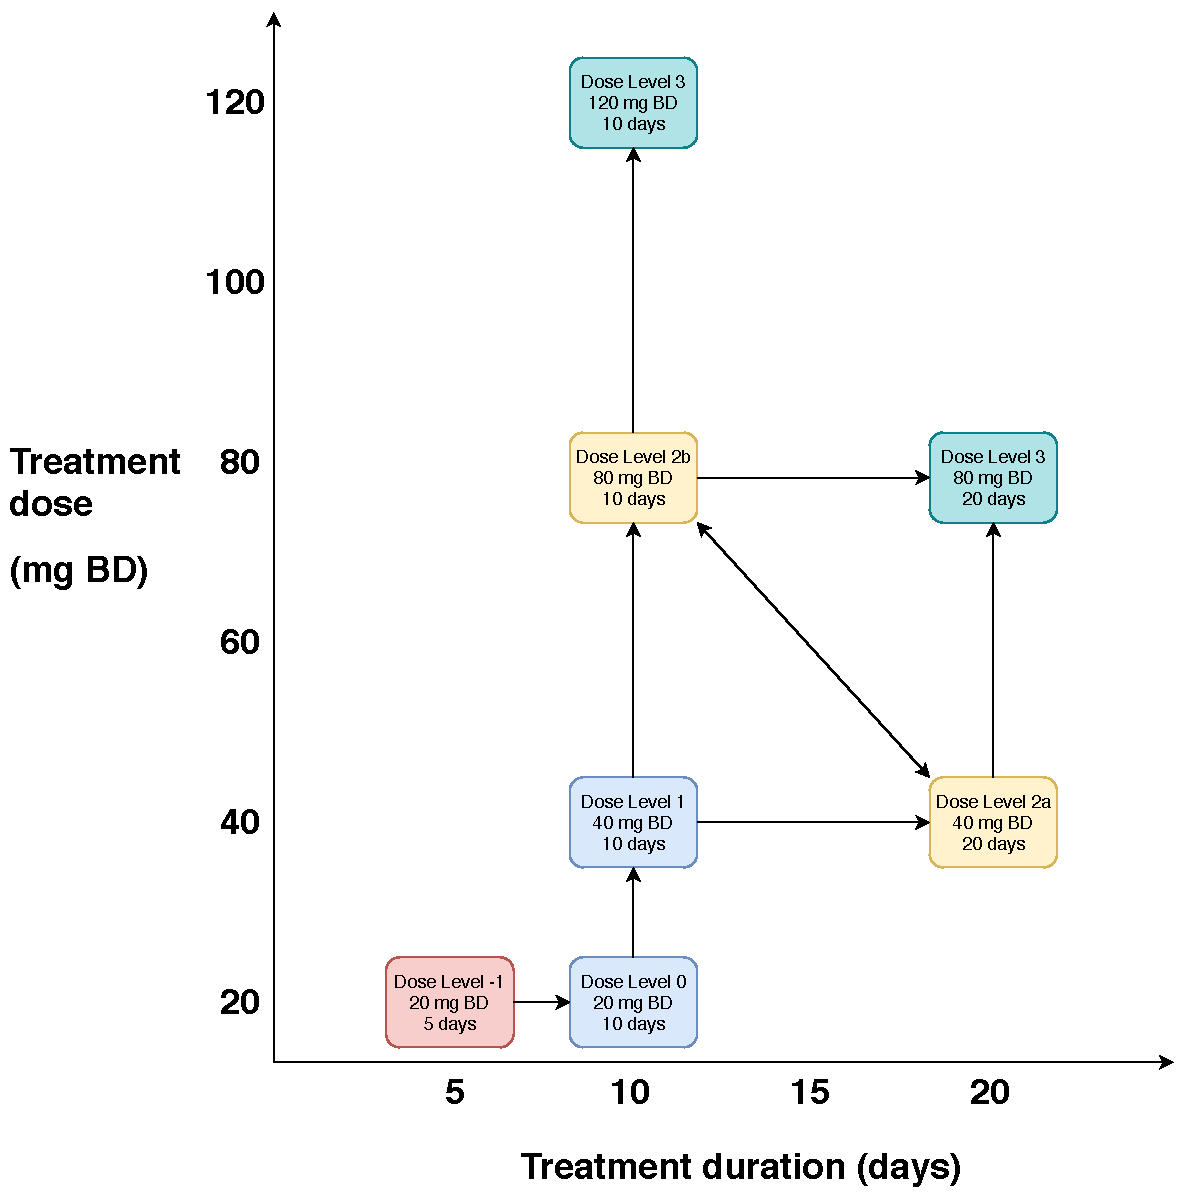
\includegraphics[width=\textwidth]{AdeptDoseCombos}
\end{figure}

Preliminary designs of the trial included only five dose levels and planned to use dose level 0 as the starting dose. During the trial design phase it was decided a new lower dose (dose level -1) would be introduced to allow for de-escalation if the initial dose was found to be too toxic. Dose escalation/de-escalation for subsequent cohorts would be determined from the two-stage PO-TITE-CRM. A two-stage design allows for escalation according to a pre-defined escalation scheme similar to a '3+3' design. The first stage dictates that if no DLT's are observed in the current cohort the dose allocated to the next cohort is the following dose in the escalation scheme. Dose levels continue to be incremented in this fashion until the first DLT is observed. In stage two, dose levels are determined by the PO-TITE-CRM.

Typically CRM designs begin by testing the first patient, or cohort, at the prior guess of TD or at a lower dose to be safe. However, clinicians may have safety concerns beginning the trial at higher dose levels as well as escalating to higher dose levels without testing lower ones. Investigators in ADePT-DDR expressed similar concerns as such a two-stage design was adopted. The escalation scheme used in stage one of ADePT-DDR will follow that of the first ordering ($d_{-1} \rightarrow d_{0} \rightarrow d_{1} \rightarrow d_{2a} \rightarrow d_{2b} \rightarrow d_{3}$). If patients in the first cohort (assigned to dose level 0) don't experience a DLT the next cohort will be allocated to dose level 1 and then if no DLTs are observed again the third cohort will be allocated to dose level 2a and so on and so forth. The dose escalation scheme was determined based on the prior probabilities of toxicity generated for each dose level.  

Information elicited from the investigators helped generate prior probabilities of toxicity for each dose level. They believed that dose level 2b would be the TD25 with 2a being less toxic. This was used in conjunction with the getprior function from the dfcrm R package \cite{cheungDfcrmDoseFindingContinual2019} which yielded priors of 0.012, 0.036, 0.084, 0.157, 0.25 and 0.355 for dose levels -1, 0, 1, 2a, 2b and 3 respectively. A half-width of 0.05 was used. Prior probabilities are also required for the plausibility of each model and even though the clinicians think that 2b will be more toxic than 2a there is no clear evidence and still a lot of uncertainty. As such it is sensible to assume a plausibility probability of 0.5 for each ordering, implying both orders are equally likely to be the true ordering of these dose levels. 

%-----------------------------------
%	SUBSECTION 3.2
%-----------------------------------
\subsection{The TITE component}
\label{section2.3.2}%first number is the chapter number, second number is section number, third is subsection etc..

The observation window for this trial will be up to a year post-treatment as the combination of radiotherapy with AZD6738 is anticipated to cause late-onset toxicity. The Acute DLT observation period is 84 days (12 weeks) post radiotherapy end with a minimum of 56 days (8 weeks) for the last patient of each cohort. However, patients will continuously be monitored for occurrence of DLT for at least 84 days (12 weeks), i.e. at least 84 days (12 weeks) from the end of radiotherapy. The full window will last for 365 days (52 weeks) post-treatment.

The TITE component incorporates a weighting contribution for each patient dependent on how long that patient has been evaluable in the study. This allows a patient to be evaluated once they have been observed for the minimum DLT period of 56 days (8 weeks). The weighting at this point is 60\% rising to 80\% at 84 days (12 weeks). A patient will not contribute fully to the model until they have completed 365 days (52 weeks) follow up (or have experienced a DLT at any stage in which case they will be weighted as a whole contribution). Linear weighting functions will be employed for any patient with a length of follow up between these three time points. One weighting function to calculate weight from 56-84 days (8-12 weeks) and another for weights from 84-365 days (12-52 weeks). For the weighting function $w(u;T)$ where $u$ is the time-to-toxicity of patient $j$ and $T$ is the time period, let $t_1, t_2, t_3$ take values 56, 84 and 365 respectively such that $T \in (t_1, t_2, t_3)$. Then for $t_1 \leq u \leq t_3$
\begin{equation}
w(u;T) = 0.6 + 0.2\frac{min(u-t_1,t_2 - t_1)}{t_2 - t_1} + 0.2\frac{max(0, u - t_2)}{t_3-t_2}.
\end{equation} 
All patients will have a minimum weight of 60\% as that is the prescribed weighting to the  minimum follow up period before dose escalation/de-escalation decisions can be made. For each additional week the patient is observed, without a DLT occurring, between weeks 8 and 12 their weighting increases by 5\%. Similarly for each week between 12 and 52 weeks, without a DLT, weighting increases by 0.5\%. Figure \ref{fig_adept:weight_function} illustrates the weight function and how the weight changes for patients dependent on how long they have been followed-up.   

\begin{figure}[h!]
	\centering
	\caption[Weight function across the follow-up period.]{Weights of patients who have not experienced a DLT across the observation window.}
	\label{fig_adept:weight_function}
	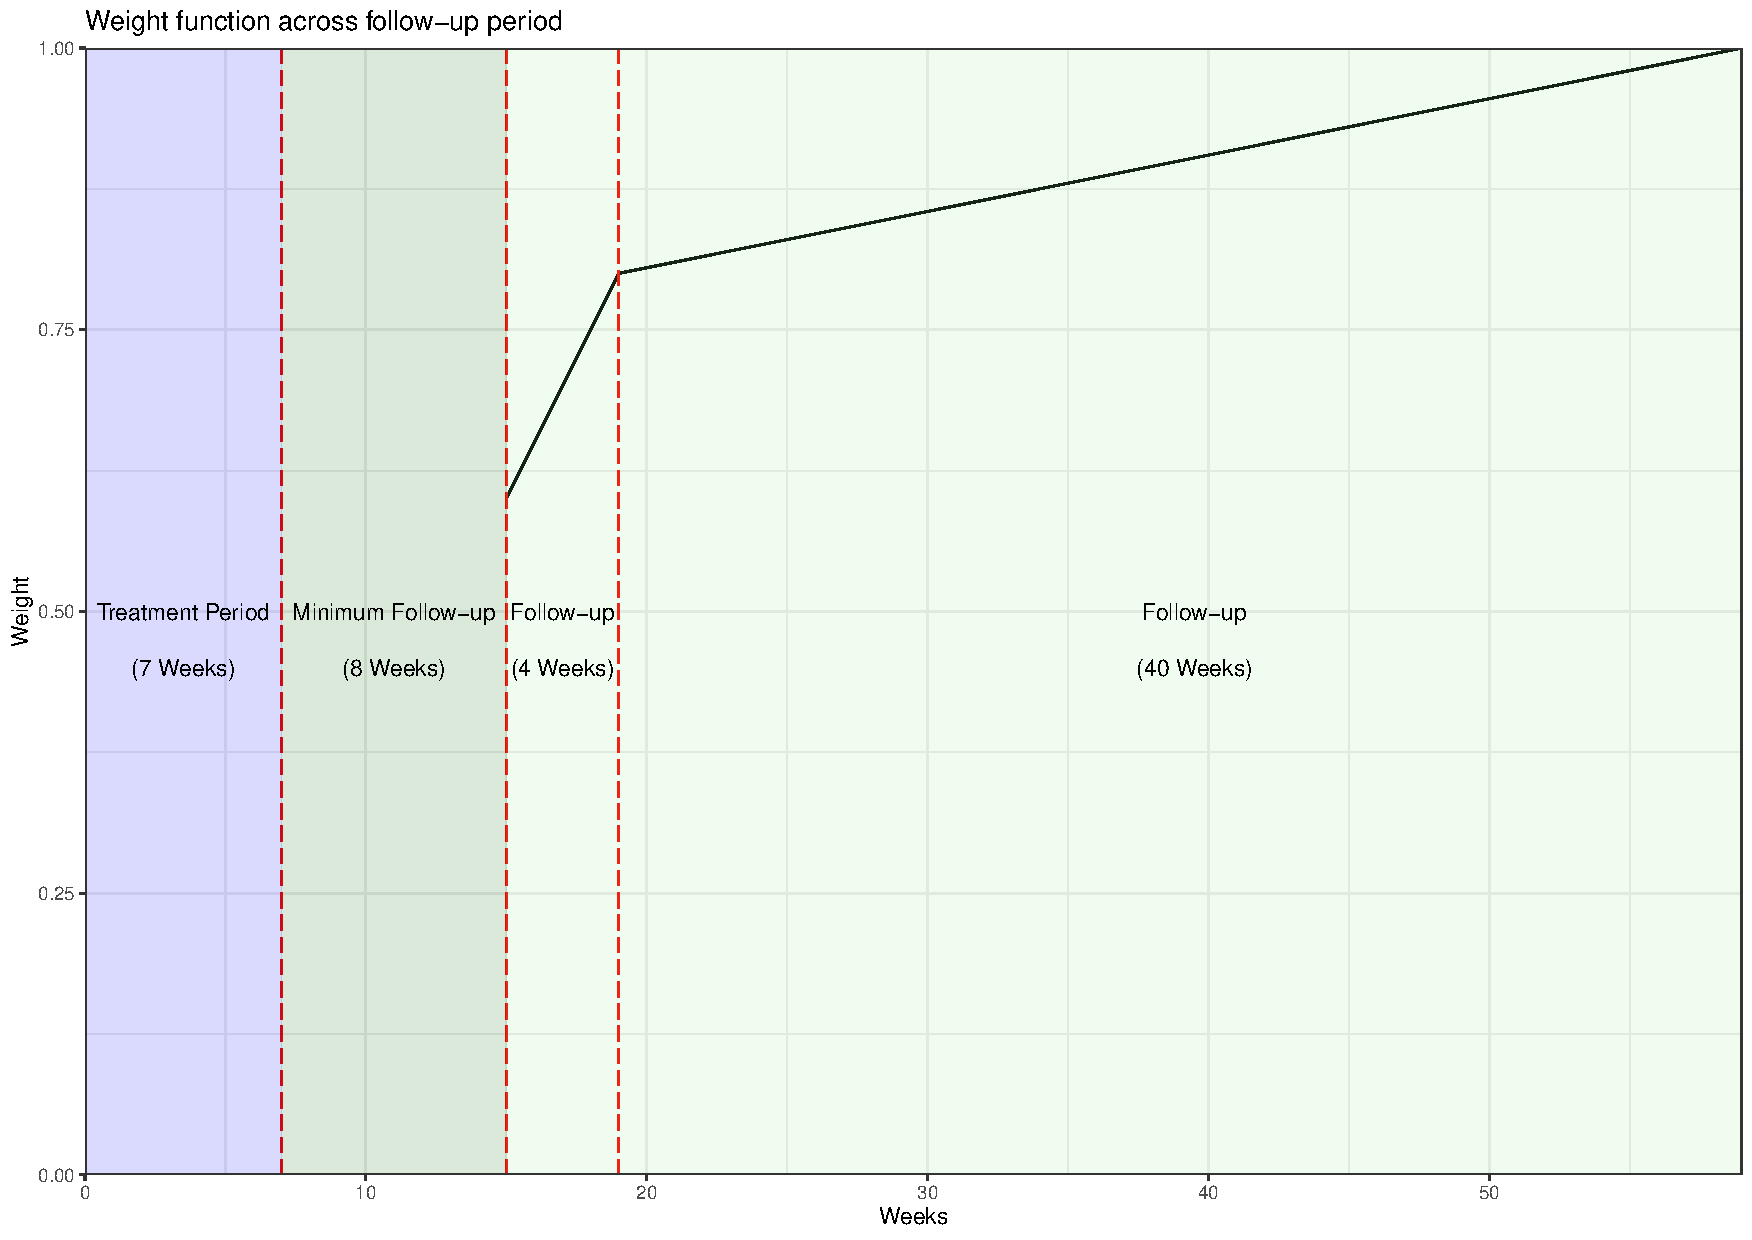
\includegraphics[width=\textwidth]{AdeptWeightFunction}
\end{figure}


The TITE-CRM originally presented by Cheung and Chappel \cite{cheungSequentialDesignsPhase2000} did not incorporate a minimum follow-up period and their design allowed for the continual recruitment of patients whenever they became available. There are some practical considerations which make this infeasible. The model would need to be run each time a new patient entered the study which requires statistical input hence the introduction of cohorts. Clinicians may also have safety concerns if we see rapid recruitment at the start of the trial and the model keeps escalating so we impose a minimum follow-up period. Initially this was set at 12 weeks (at 80\% weighting) however, statisticians AP and PG  pointed out that dose escalation/de-escalation decisions would have to take place 19 weeks (7 weeks treatment and 12 weeks follow-up) after recruitment of the third patient in the cohort. Dependent on the recruitment rates this could extend the duration of the trial and negates the benefits of using a TITE design. The investigators aslo agreed this was too long and settled on lowering this period to 8 weeks (at 60\% weighting) whilst also including the original 12 week weighting of 80\%.

%Additional rules were implemented into the design for safety and early stopping.  
%Additional 
%
%Further considerations were made

%-----------------------------------
%	SUBSECTION 3.3
%-----------------------------------
\subsection{Stopping Rules}
\label{section2.3.3}%first number is the chapter number, second number is section number, third is subsection etc..

A practical modification was included to allow for early stopping of the trial if there is sufficient evidence that the TD has been reached. Sufficient evidence is achieved once 15 patients (five cohorts) have been treated at the same dose level and the model allocates that dose level again to a sixth cohort. This rule evolved from the original designs of the trial which involved 30 patients with a dose expansion cohort to ensure at least 15 patients were treated at the TD. 

Initial simulations highlighted the inadequacy of these design parameters as operating characteristics for various scenarios were poor, specifically in terms of correct TD selection. Clinicians explained the inclusion of the dose expansion cohort was to ensure the dose-finding aspect of the trial did not take a large amount of time whilst also allowing safety to be assessed at the TD. In order to ensure that a reasonable amount of patients would be treated at the TD, the trial wouldn't take longer than necessary and operating characteristics improved, the sample size was increase and this rule was introduced.

A rule was also implemented to allow for early termination of the trial in the case of excess toxicity at the lowest dose. If the posterior probability of DLT at the lowest dose is higher than 0.35 with a probability of 80\% and has been tested the trials safety committee will be alerted and will recommend if the trial should be stopped. As the trial starts at dose level 0, which is not the lowest dose, it is possible for the trial to recommend terminating without ever allocating patients to the lowest dose level. As such it was decided early termination would only occur once at least 3 patients (1 cohort) have been allocated dose level -1. 

%-----------------------------------
%	SUBSECTION 3.
%-----------------------------------
\subsection{Operating Characteristics}
\label{section2.3.4}%first number is the chapter number, second number is section number, third is subsection etc.. 

Simulations were continually utilised during the design process of the trial to assess how various changes impact the overall performance. These changes to design features such as the sample size, weight function and stopping rules helped inform decisions which led to the final design.  

Functions from pocrm package in R \cite{wagesPocrmRpackagePhase2013, wagesPocrmDoseFinding2019} were modified in order to perform simulations and conduct the trial. The majority of work involved integrating the TITE component and the stopping rules into the code. In standard CRM designs a binary outcome for toxicity is generated for each patient based on a pre-specified true DLT rates for the dose they are assigned. Adding the TITE component means the time the toxicity occurs also has to be generated, the simulation must also track this time and incorporate this information into the PO-TITE-CRM model when it needs to make dose allocation decisions for the next cohort. We defined multiple scenarios to reflect various real life possibilities in order to assess the designs performance.  

Standard scenarios to run involve adjusting the true DLT rates to reflect each dose being the TD25. For each of these we calculate the probability of selecting each dose as the TD25. It would be expected the dose with the highest probability of being selected has its true DLT rate set at 25\% to match the target rate. A high probability of selection for the correct dose implies the design works well in the specified scenario. Additional characteristics such as the average number of patients at each dose level are also investigated. This can be used to look at how many patients may potentially be allocated to a toxic dose. It is also necessary to consider performance when all doses are too toxic, here we would want the design to recommend stopping early. Usually the true DLT rates used to define these scenarios abide by the monotonicity assumption. Due to the partial ordering we consider scenarios in which the true DLT rates follow both orders. For trials with a large amount of orders it may be unfeasible to run so many simulations. However, as ADePT-DDR only has two orders we explored all scenarios for each ordering.

We simulated 2000 trials for each scenario using the finalised design detailed in section \ref{section2.3}. Simulations were based on the assumption that the trial would recruit one patient per month. The occurrence of DLT's were randomly generated for patients in each cohort using a Bernoulli distribution with the probability set at the true DLT rate for the cohorts assigned dose level in the specific scenario. For patients who had a DLT occur, the time at which the DLT occurred was randomly generated using a uniform distribution which spanned the start of treatment to the end of follow-up.  

Table \ref{tab_adept:OCorder1} details simulations for eight scenarios to test the performance of the PO-TITE-CRM design using true DLT rates which reflect the first ordering. We analyse scenarios where each dose is the TD25 (scenarios 1-6) and when all doses are too toxic (scenario 8). Additionally, we also investigate performance under conditions where the probability of DLT is fairly similar between doses (scenario 7). This is a notoriously difficult circumstance for CRM designs to deal with as the limited number of patients and events at each dose make it hard to accurately estimate toxicity probabilities if they are similar. Simulation results for ordering 2 are shown in Table \ref{tab_adept:OCorder2} where dose level 2a is considered more toxic than 2b. This is achieved by altering the true DLT rates so 2b has a lower probability of DLT compared to 2a. 

Ideally we want the probability of selection for the dose allocated at TD25 to be as high as possible and greater than other dose levels. For scenarios 1-7 the TD25 is highlighted in bold along with results from the simulations. However, for scenario 8 where all doses are too toxic we expect the trial to terminate early, here 'stop' should be selected and its associated probability of stopping is shown in bold. 

In scenarios 1 - 6 (Table \ref{tab_adept:OCorder1}), this design correctly selects the TD25 with probabilities between 44\% and 79\%, under the assumption 2b is more toxic than 2a. Likewise, for the ordering where 2a is more toxic than 2b, scenarios 9-14 (Table \ref{tab_adept:OCorder2}) have probabilities between 43\% and 78\% of correctly selecting the TD25. Correct selection probabilities are generally higher when the TD25 is at the first and last dose levels compared to dose levels 2a and 2b. However, these dose levels are still chosen with the highest probability as the TD25 in their given scenarios. For scenarios 7 and 15, the probabilities of toxicity are equally spaced, approximately 5\% apart. This is a relatively diffcult scenario for dose-finding studies to handle. The probability of selecting the TD25 is 26\% and 30\% for orderings 1 and 2 respectively. In scenarios 8 and 16, where all the doses are too toxic, the design very seldom allocates patients higher than the first three doses and there is a high chance (73\%) that the trial will recommend early stopping.



\begin{table}[h!] % OC for order 1 
	
	\caption[Operating Characteristics for ordering 1.]{\label{tab_adept:OCorder1} Operating Characteristics of the two-stage PO-TITE-CRM (with true DLT rates that imply 2b is more toxic than 2a) based on 2000 simulated trials. Definitions: DLT: Dose-limiting toxicity. P(select):
	Probability of selecting a dose as the TD25.}
	\centering
	\begin{singlespace}
	\resizebox{\linewidth}{!}{
		\begin{tabular}[t]{ccccccccc}
			\toprule
			\multicolumn{2}{c}{ } & \multicolumn{6}{c}{Dose Levels} \\
			\cmidrule(l{3pt}r{3pt}){3-8}
			&  & -1 & 0 & 1 & 2a & 2b & 3 & Stop\\
			\midrule
			Scenario & Prior DLT & 0.01 & 0.04 & 0.08 & 0.16 & 0.25 & 0.35 & \\
			\cmidrule{1-9}
			\rowcolor{gray!6}   & True DLT rate & \textbf{0.25} & 0.4 & 0.45 & 0.5 & 0.55 & 0.6 & \\
			
			\rowcolor{gray!6}   & P(select) & \textbf{0.67} & 0.18 & 0.05 & 0 & 0 & 0 & 0.10\\
			
			\rowcolor{gray!6}   & \% of patients & \textbf{39} & 32 & 21 & 6 & 3 & 0 & \\
			
			\rowcolor{gray!6}  \multirow{-4}{*}{\centering\arraybackslash 1: TD25 @-1} & Mean number of patients & \textbf{10.03} & 8.26 & 5.34 & 1.65 & 0.68 & 0.06 & \\
			\cmidrule{1-9}
			& True DLT rate & 0.12 & \textbf{0.25} & 0.4 & 0.45 & 0.5 & 0.55 & \\
			
			& P(select) & 0.23 & \textbf{0.51} & 0.2 & 0.03 & 0.02 & 0 & 0.01\\
			
			& \% of patients & 17 & \textbf{35} & 29 & 11 & 6 & 1 & \\
			
			\multirow{-4}{*}{\centering\arraybackslash 2: TD25 @0} & Mean number of patients & 5.19 & \textbf{10.49} & 8.74 & 3.31 & 1.77 & 0.28 & \\
			\cmidrule{1-9}
			\rowcolor{gray!6}   & True DLT rate & 0.09 & 0.12 & \textbf{0.25} & 0.4 & 0.45 & 0.5 & \\
			
			\rowcolor{gray!6}   & P(select) & 0.01 & 0.2 & \textbf{0.54} & 0.14 & 0.1 & 0.01 & 0\\
			
			\rowcolor{gray!6}   & \% of patients & 4 & 21 & \textbf{35} & 22 & 16 & 3 & \\
			
			\rowcolor{gray!6}  \multirow{-4}{*}{\centering\arraybackslash 3: TD25 @1} & Mean number of patients & 1.2 & 6.63 & \textbf{10.99} & 7.08 & 4.93 & 0.97 & \\
			\cmidrule{1-9}
			& True DLT rate & 0.06 & 0.09 & 0.12 & \textbf{0.25} & 0.4 & 0.45 & \\
			
			& P(select) & 0 & 0.01 & 0.21 & \textbf{0.5} & 0.23 & 0.04 & 0\\
			
			& \% of patients & 2 & 12 & 20 & \textbf{32} & 25 & 11 & \\
			
			\multirow{-4}{*}{\centering\arraybackslash 4: TD25 @2a} & Mean number of patients & 0.5 & 3.84 & 6.61 & \textbf{10.66} & 8.16 & 3.5 & \\
			\cmidrule{1-9}
			\rowcolor{gray!6}   & True DLT rate & 0.03 & 0.06 & 0.09 & 0.12 & \textbf{0.25} & 0.4 & \\
			
			\rowcolor{gray!6}   & P(select) & 0 & 0 & 0.03 & 0.29 & \textbf{0.44} & 0.25 & 0\\
			
			\rowcolor{gray!6}   & \% of patients & 1 & 10 & 12 & 24 & \textbf{28} & 25 & \\
			
			\rowcolor{gray!6}  \multirow{-4}{*}{\centering\arraybackslash 5: TD25 @2b} & Mean number of patients & 0.22 & 3.39 & 4.18 & 8.13 & \textbf{9.42} & 8.33 & \\
			\cmidrule{1-9}
			& True DLT rate & 0.01 & 0.03 & 0.06 & 0.09 & 0.12 & \textbf{0.25} & \\
			
			& P(select) & 0 & 0 & 0 & 0.09 & 0.12 & \textbf{0.79} & 0\\
			
			& \% of patients & 0 & 10 & 11 & 17 & 18 & \textbf{43} & \\
			
			\multirow{-4}{*}{\centering\arraybackslash 6: TD25 @3} & Mean number of patients & 0.1 & 3.12 & 3.49 & 5.35 & 5.51 & \textbf{13.48} & \\
			\cmidrule{1-9}
			\rowcolor{gray!6}   & True DLT rate & 0.05 & 0.1 & 0.15 & 0.2 & \textbf{0.25} & 0.3 & \\
			
			\rowcolor{gray!6}   & P(select) & 0 & 0.03 & 0.14 & 0.31 & \textbf{0.26} & 0.26 & 0\\
			
			\rowcolor{gray!6}   & \% of patients & 2 & 13 & 19 & 25 & \textbf{22} & 19 & \\
			
			\rowcolor{gray!6}  \multirow{-4}{*}{\centering\arraybackslash 7: Equal steps in DLT rate} & Mean number of patients & 0.6 & 4.11 & 5.88 & 8.02 & \textbf{6.95} & 5.9 & \\
			\cmidrule{1-9}
			& True DLT rate & 0.5 & 0.6 & 0.65 & 0.7 & 0.75 & 0.8 & \\
			
			& P(select) & 0.26 & 0 & 0 & 0 & 0 & 0 & \textbf{0.74}\\
			
			& \% of patients & 56 & 27 & 15 & 2 & 0 & 0 & \\
			
			\multirow{-4}{*}{\centering\arraybackslash 8: All  toxic} & Mean number of patients & 8.61 & 4.17 & 2.28 & 0.28 & 0.03 & 0 & \\
			\bottomrule
	\end{tabular}}
\end{singlespace}
\end{table}

\begin{table}[h!] % OC for order 2
	
	\caption[Operating Characteristics for ordering 2.]{\label{tab_adept:OCorder2}  Operating Characteristics of the two-stage PO-TITE-CRM (with true DLT rates that imply 2a is more toxic than 2b) based on 2000 simulated trials. Definitions: DLT: Dose-limiting toxicity. P(select): Probability of selecting a dose as the TD25.}
	\centering
	\begin{singlespace}
	\resizebox{\linewidth}{!}{
		\begin{tabular}[t]{ccccccccc}
			\toprule
			\multicolumn{2}{c}{ } & \multicolumn{6}{c}{Dose Levels} \\
			\cmidrule(l{3pt}r{3pt}){3-8}
			&  & -1 & 0 & 1 & 2a & 2b & 3 & Stop\\
			\midrule
			Scenario & Prior DLT & 0.01 & 0.04 & 0.08 & 0.16 & 0.25 & 0.35 & \\
			\cmidrule{1-9}
			\rowcolor{gray!6}   & True DLT rate & \textbf{0.25} & 0.4 & 0.45 & 0.55 & 0.5 & 0.6 & \\
			
			\rowcolor{gray!6}   & P(select) & \textbf{0.69} & 0.18 & 0.04 & 0 & 0 & 0 & 0.08\\
			
			\rowcolor{gray!6}   & \% of patients & \textbf{39} & 33 & 20 & 6 & 2 & 0 & \\
			
			\rowcolor{gray!6}  \multirow{-4}{*}{\centering\arraybackslash 9: TD25 @-1} & Mean number of patients & \textbf{10.29} & 8.57 & 5.24 & 1.44 & 0.51 & 0.04 & \\
			\cmidrule{1-9}
			& True DLT rate & 0.12 & \textbf{0.25} & 0.4 & 0.5 & 0.45 & 0.55 & \\
			
			& P(select) & 0.23 & \textbf{0.53} & 0.19 & 0.02 & 0.02 & 0 & 0.01\\
			
			& \% of patients & 18 & \textbf{36} & 30 & 10 & 6 & 1 & \\
			
			\multirow{-4}{*}{\centering\arraybackslash 10: TD25 @0} & Mean number of patients & 5.17 & \textbf{10.77} & 8.76 & 2.99 & 1.66 & 0.18 & \\
			\cmidrule{1-9}
			\rowcolor{gray!6}   & True DLT rate & 0.09 & 0.12 & \textbf{0.25} & 0.45 & 0.4 & 0.5 & \\
			
			\rowcolor{gray!6}   & P(select) & 0.02 & 0.2 & \textbf{0.58} & 0.08 & 0.11 & 0.01 & 0\\
			
			\rowcolor{gray!6}   & \% of patients & 4 & 21 & \textbf{36} & 20 & 16 & 3 & \\
			
			\rowcolor{gray!6}  \multirow{-4}{*}{\centering\arraybackslash 11: TD25 @1} & Mean number of patients & 1.25 & 6.55 & \textbf{11.48} & 6.48 & 5.12 & 0.82 & \\
			\cmidrule{1-9}
			& True DLT rate & 0.06 & 0.09 & 0.12 & \textbf{0.25} & 0.15 & 0.45 & \\
			
			& P(select) & 0 & 0.02 & 0.09 & \textbf{0.43} & 0.33 & 0.13 & 0\\
			
			& \% of patients & 1 & 11 & 16 & \textbf{30} & 23 & 18 & \\
			
			\multirow{-4}{*}{\centering\arraybackslash 12: TD25 @2a} & Mean number of patients & 0.42 & 3.84 & 5.32 & \textbf{10.22} & 7.9 & 6 & \\
			\cmidrule{1-9}
			\rowcolor{gray!6}   & True DLT rate & 0.03 & 0.06 & 0.09 & 0.35 & \textbf{0.25} & 0.4 & \\
			
			\rowcolor{gray!6}   & P(select) & 0 & 0 & 0.14 & 0.32 & \textbf{0.43} & 0.11 & 0\\
			
			\rowcolor{gray!6}   & \% of patients & 1 & 11 & 18 & 29 & \textbf{27} & 14 & \\
			
			\rowcolor{gray!6}  \multirow{-4}{*}{\centering\arraybackslash 13: TD25 @2b} & Mean number of patients & 0.28 & 3.57 & 6.06 & 9.72 & \textbf{9.01} & 4.48 & \\
			\cmidrule{1-9}
			& True DLT rate & 0.01 & 0.03 & 0.06 & 0.12 & 0.09 & \textbf{0.25} & \\
			
			& P(select) & 0 & 0 & 0 & 0.13 & 0.09 & \textbf{0.78} & 0\\
			
			& \% of patients & 0 & 10 & 11 & 20 & 16 & \textbf{42} & \\
			
			\multirow{-4}{*}{\centering\arraybackslash 14: TD25 @3} & Mean number of patients & 0.08 & 3.11 & 3.46 & 6.04 & 5.04 & \textbf{13.05} & \\
			\cmidrule{1-9}
			\rowcolor{gray!6}   & True DLT rate & 0.05 & 0.1 & 0.15 & \textbf{0.25} & 0.2 & 0.3 & \\
			
			\rowcolor{gray!6}   & P(select) & 0 & 0.02 & 0.14 & \textbf{0.3} & 0.28 & 0.26 & 0\\
			
			\rowcolor{gray!6}   & \% of patients & 2 & 13 & 19 & \textbf{27} & 22 & 18 & \\
			
			\rowcolor{gray!6}  \multirow{-4}{*}{\centering\arraybackslash 15: Equal steps in DLT rate} & Mean number of patients & 0.61 & 4.11 & 6.13 & \textbf{8.56} & 6.88 & 5.59 & \\
			\cmidrule{1-9}
			& True DLT rate & 0.5 & 0.6 & 0.65 & 0.75 & 0.7 & 0.8 & \\
			
			& P(select) & 0.27 & 0 & 0 & 0 & 0 & 0 & \textbf{0.73}\\
			
			& \% of patients & 56 & 27 & 15 & 2 & 0 & 0 & \\
			
			\multirow{-4}{*}{\centering\arraybackslash 16: All  toxic} & Mean number of patients & 8.78 & 4.26 & 2.35 & 0.3 & 0.02 & 0 & \\
			\bottomrule
	\end{tabular}}
\end{singlespace}
\end{table}
 

Additionally, we assess designs based on how doses are allocated to patients. Designs may correctly select the TD however, this could be undesirable and unethical if the majority of patients are over dosed at the more toxic dose levels. The average number and the percentage of patients at each dose level, for each scenario, is recorded in Tables \ref{tab_adept:OCorder1} and \ref{tab_adept:OCorder2}. 

The percentage of patients treated at the TD25 ranges between 27\% and 43\% for each scenario under both orderings. The design also allocates the most patients on average to the TD25 apart from in scenario 7. In this case more patients were allocated to the next lowest dose, we have already discussed the difficulties of this scenario so this characteristic is not too concerning. The mean number of patients recruited for scenarios 1-6 is 26, 30, 32, 33, 34 and 31 respectively. Similarly for scenarios 9-14 its 26, 30, 32, 34, 33 and 31. Even though we allow for up to 60 patients the majority of trials terminate early based on the pre-defined rules for selecting the TD25.

Overall, the simulation results show the specification of this design performs relatively well in a number of scenarios. We have shown there is a high probability of the trial stopping early if all dose-levels are too toxic. We have also shown the design behaves in an appropriate manner when there is a lack of disparity between dose-levels in terms of toxicity. Finally, we have demonstrated that regardless of the ordering we observe the PO-TITE-CRM has a high probability of selecting the correct dose. There are a number of limitations to the operating characteristics presented here which are due to the specification of the simulations and trial design. Section \ref{section2.4} explores and discusses these limitations in more detail.

%----------------------------------------------------------------------------------------
%	SECTION 4
%-------------------------.

\section{Inspection of the operating characteristics}  
\label{section2.4}%first number is the chapter number, second number is section number, third is subsection etc.. 

The operating characteristics presented in section \ref{section2.3.4} provide an insight into how the trial design operates and its effectiveness at selecting the TD25. However, there are a number of factors which impact the results seen here. These factors can be grouped into two main categories, limitations with the simulations performed or the trial design.

In order to simulate various scenarios the true DLT rates are adjusted to reflect the TD25 being at different dose levels. There is no formal process to select these values as such their selection is fairly arbitrary. We set one dose level as the TD25 with lower and higher dose levels set at lower and higher DLT rates respectively. Figure \ref{fig_adept:dlt_rates} illustrates the dose levels for scenarios in Table \ref{tab_adept:OCorder1} where dose level 2b is more toxic than 2a. The DLT rates cover a number of possible scenarios and accounts for a range of plausible values. However, these true DLT rates may not accurately reflect what we observe once the trial begins. Also, the relationship between the rates and the dose levels may not be similar to what we use in the simulations. Multiple other scenarios could be investigated but it would still be impossible to account for all possible scenarios which may occur. Hence when evaluating the performance of a design its important to note the scenario in which its being evaluated and whether or not the design performs as expected and to an adequate level. For ADePT-DDR, the design is producing reasonable characteristics under each scenario. 

\begin{figure}[h!]
	\centering
	\caption[Illustration of true DLT rates used in simulations.]{True DLT rates used for each of the scenarios where dose level 2b is more toxic than 2a. The dotted red line represents the target dlt rate of 25\% (TD25).}
	\label{fig_adept:dlt_rates}
	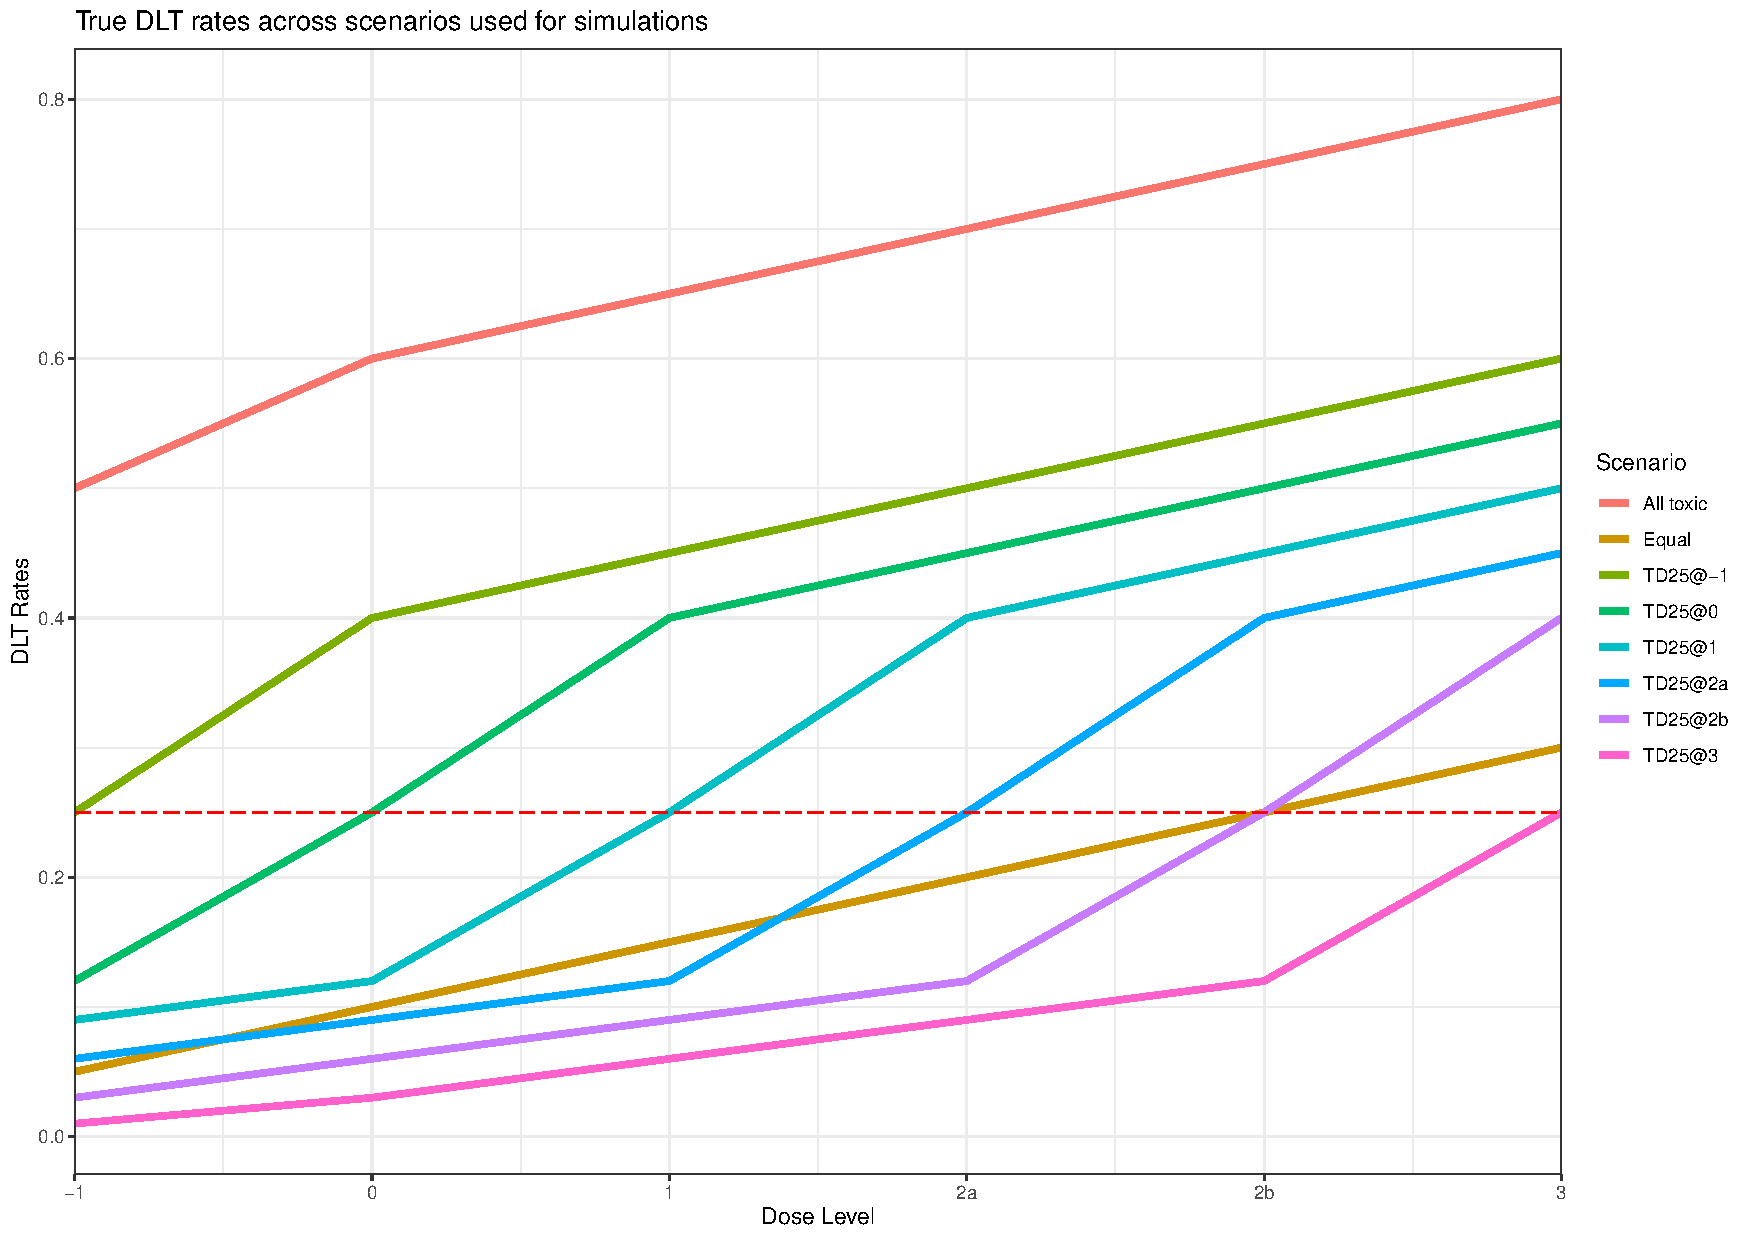
\includegraphics[width=\textwidth]{AdeptDLTRates}
\end{figure}
 
The original methodological papers by Wages et al. \cite{wagesUsingTimetoeventContinual2013,wagesContinualReassessmentMethod2011} only provide simulations for their examples using true DLT rates that are monotonically increasing which represented one of their possible orderings. We cannot tell how their design would perform under scenarios from different orderings. It is unclear as to why this wasn't examined. To begin with in ADePT-DDR we followed suit and only produced simulations under a monotonically increasing DLT rate (order where 2b is more toxic than 2a, Table \ref{tab_adept:OCorder1}).However, as we are unclear on the ordering of 2a and 2b there is a possibility that 2b is less toxic meaning the simulations produced thus far would not be an accruate assessment of how the design performs. This was the main motivation for running scenarios in Table \ref{tab_adept:OCorder2}, in which we see the design performs at a similar level regardless of ordering. ADePT-DDR is a simple case of partial ordering as there are only two possible orderings and six dose-levels. For trials with higher numbers of orderings or dose-levels the number of scenarios which would have to be evaluated would increase and may not be feasible. Here it may be more beneficial to choose a handful of scenarios from multiple different orderings to cover a wider range of possible outcomes for the trial to assess the design. 

Another limitation with the simulations is the way in which the time-to-event data is generated. The time of DLTs is sampled from a uniform distribution $U(0, 413)$, where the time of the DLT can occur at any time between the patient beginning treatment and the end of follow-up (413 days). Using this uniform distribution implies that a DLT has equal probability of occuring at any time-point in the observation window. This may not be an accurate representation of what happens in the actual trial. Similar comments can be made about the accrual rate used in the simulations. Here we specified the recruitment of one patient per month which is in no way guaranteed for the actual trial. The simulations are also able to instantaneously determine dose-levels for incoming cohorts with all available information. This does not fully reflect the process in which dose-escalation decisions would be made during the actual running of the trial. Analysis would require a data snapshot and time would have to be spent cleaning the data and determining the next dose-level. Meaning any data from the point of the snapshot would not be included in any dose escalation/de-escalation decisions. 

There are a number of features in this trial design which may impact how it performs. The partial ordering caused by dose levels 2a and 2b adds complexity to design. If one of these dose-levels were to be removed or a normal ordering was assumed a standard TITE-CRM design could be used instead. However, this would take away from what the trial was trying to discover. This trial also has a long follow-up period due to potential late-onset toxicities and in turn will have a long duration. The TITE component will allow for the duration to be a lot shorter than it would be otherwise. TITE-CRM designs allow for patients to be recruited sequentially and allocated a dose based on available information from patients all ready in the trial. The design for ADePT-DDR uses cohorts of three and a minimum follow-up period. The dose-escalation decisions will only be made every third patient after a specific amount of time. This is done for safety and practicality reasons but means that some patients may not be able to enter the trial and it also loses some of the benefits of the TITE-CRM. We also have a sample size of 60 patients but include a stopping rule for when a consensus is reached which means we often don't recruit the maximum sample size. Further simulations were produced to investigate how these features affected the trial. Table \ref{tab_adept:Design_Comparison} compares selection probabilities from the ADePT-DDR trial design (Table \ref{tab_adept:OCorder1}) with five alternative designs. 
 
\begin{enumerate}
	\item TITE-CRM design. This design assumes a that partial ordering doesn't exist and that dose-level 2b is more toxic than 2a. A TITE-CRM is used instead of a PO-TITE-CRM. All other stopping rules and details remain the same. 
	\item PO (Partial Ordering design). This design removes the TITE component and uses a PO-CRM as detailed by \cite{wagesContinualReassessmentMethod2011}. This requires the removal of the minimum follow-up period so all dose allocation decisions are made once all 3 patients in a cohort have been observed for the full follow-up period of one year. All other stopping rules and details remain the same. 
	\item N = 30. This design uses a fixed sample size of 30 patients and removes the stopping rule for reaching consensus. Analysis is still conducted using the PO-TITE-CRM. All other stopping rules and details remain the same. 
	\item N = 60. This design uses a fixed sample size of 60 patients and removes the stopping rule for reaching consensus. Analysis is still conducted using the PO-TITE-CRM. All other stopping rules and details remain the same. 
	\item No follow-up (No FU). This design uses a cohort size of 1 and removes the minimum follow-up period. All other stopping rules remain the same. \textbf{Simulation results for this design are incorrect. Please ignore for now.}
\end{enumerate} 


\begin{table}
	
	\caption[Selection probabilities for alternative designs.]{\label{tab_adept:Design_Comparison}Selection probabilities of the TD25 and expected trial duration (in months) for the PO-TITE, TITE and PO-CRM designs as well as modified PO-TITE-CRM designs for scenarios 1-8 based on 2000 simulated trials.}
	
	\centering
	\begin{singlespace}
		\resizebox{\linewidth}{!}{
			\fontsize{12}{11}\selectfont
			\begin{tabular}[t]{ccccccccccc}
				\toprule
				\multicolumn{3}{c}{ } & \multicolumn{6}{c}{Dose Levels} \\
				\cmidrule(l{3pt}r{3pt}){4-9}
				&  &  & -1 & 0 & 1 & 2a & 2b & 3 & Stop & Duration\\
				\midrule
				Scenario & CRM details & Prior DLT & 0.01 & 0.04 & 0.08 & 0.16 & 0.25 & 0.35 &  & \\
				\cmidrule{1-11}
				\rowcolor{gray!6}   &  & True DLT rate & 0.25 & 0.4 & 0.45 & 0.5 & 0.55 & 0.6 &  & \\
				
				\rowcolor{gray!6}   & PO-TITE & P(select) & 0.67 & 0.18 & 0.05 & 0 & 0 & 0 & 0.1 & 64.41\\
				
				\rowcolor{gray!6}   & TITE & P(select) & 0.69 & 0.21 & 0.06 & 0.01 & 0 & 0 & 0.04 & 66.82\\
				
				\rowcolor{gray!6}   & PO & P(select) & 0.57 & 0.18 & 0.04 & 0.01 & 0 & 0 & 0.2 & 131.02\\
				
				\rowcolor{gray!6}   & N = 30 & P(select) & 0.67 & 0.19 & 0.04 & 0.01 & 0 & 0 & 0.09 & 66.75\\
				
				\rowcolor{gray!6}   & N = 60 & P(select) & 0.77 & 0.13 & 0.01 & 0 & 0 & 0 & 0.09 & 122.06\\
				
				\rowcolor{gray!6}  \multirow{-7}{*}{\centering\arraybackslash 1: TD25 @-1} & No FU & P(select) & 0.6 & 0.22 & 0.07 & 0.02 & 0.01 & 0 & 0.08 & 44.51\\
				\cmidrule{1-11}
				&  & True DLT rate & 0.12 & 0.25 & 0.4 & 0.45 & 0.5 & 0.55 &  & \\
				
				& PO-TITE & P(select) & 0.23 & 0.51 & 0.2 & 0.03 & 0.02 & 0 & 0.01 & 72.42\\
				
				& TITE & P(select) & 0.2 & 0.56 & 0.2 & 0.04 & 0 & 0 &  & 71.43\\
				
				& PO & P(select) & 0.21 & 0.53 & 0.2 & 0.02 & 0.01 & 0 & 0.02 & 163.6\\
				
				& N = 30 & P(select) & 0.22 & 0.5 & 0.22 & 0.02 & 0.02 & 0 & 0.01 & 72.13\\
				
				& N = 60 & P(select) & 0.14 & 0.72 & 0.13 & 0.01 & 0 & 0 & 0.01 & 134.39\\
				
				\multirow{-7}{*}{\centering\arraybackslash 2: TD25 @0} & No FU & P(select) & 0.2 & 0.47 & 0.21 & 0.05 & 0.04 & 0.01 & 0.02 & 45.99\\
				\cmidrule{1-11}
				\rowcolor{gray!6}   &  & True DLT rate & 0.09 & 0.12 & 0.25 & 0.4 & 0.45 & 0.5 &  & \\
				
				\rowcolor{gray!6}   & PO-TITE & P(select) & 0.01 & 0.2 & 0.54 & 0.14 & 0.1 & 0.01 &  & 76.69\\
				
				\rowcolor{gray!6}   & TITE & P(select) & 0.01 & 0.21 & 0.54 & 0.2 & 0.03 & 0.01 &  & 72.95\\
				
				\rowcolor{gray!6}   & PO & P(select) & 0.02 & 0.16 & 0.59 & 0.14 & 0.08 & 0.01 &  & 179.11\\
				
				\rowcolor{gray!6}   & N = 30 & P(select) & 0.01 & 0.19 & 0.52 & 0.15 & 0.12 & 0 &  & 72.72\\
				
				\rowcolor{gray!6}   & N = 60 & P(select) & 0 & 0.13 & 0.71 & 0.1 & 0.06 & 0 &  & 136.33\\
				
				\rowcolor{gray!6}  \multirow{-7}{*}{\centering\arraybackslash 3: TD25 @1} & No FU & P(select) & 0.03 & 0.18 & 0.48 & 0.15 & 0.12 & 0.03 & 0.01 & 45.66\\
				\cmidrule{1-11}
				&  & True DLT rate & 0.06 & 0.09 & 0.12 & 0.25 & 0.4 & 0.45 &  & \\
				
				& PO-TITE & P(select) & 0 & 0.01 & 0.21 & 0.5 & 0.23 & 0.04 &  & 79.8\\
				
				& TITE & P(select) & 0 & 0.01 & 0.21 & 0.57 & 0.17 & 0.03 &  & 76.37\\
				
				& PO & P(select) & 0 & 0.02 & 0.21 & 0.49 & 0.22 & 0.05 &  & 190.17\\
				
				& N = 30 & P(select) & 0 & 0.01 & 0.22 & 0.46 & 0.26 & 0.04 &  & 72.8\\
				
				& N = 60 & P(select) & 0 & 0 & 0.17 & 0.64 & 0.18 & 0.01 &  & 136.56\\
				
				\multirow{-7}{*}{\centering\arraybackslash 4: TD25 @2a} & No FU & P(select) & 0.02 & 0.02 & 0.22 & 0.42 & 0.23 & 0.09 &  & 43.57\\
				\cmidrule{1-11}
				\rowcolor{gray!6}   &  & True DLT rate & 0.03 & 0.06 & 0.09 & 0.12 & 0.25 & 0.4 &  & \\
				
				\rowcolor{gray!6}   & PO-TITE & P(select) & 0 & 0 & 0.03 & 0.29 & 0.44 & 0.25 &  & 80.69\\
				
				\rowcolor{gray!6}   & TITE & P(select) & 0 & 0 & 0.02 & 0.23 & 0.55 & 0.19 &  & 77.92\\
				
				\rowcolor{gray!6}   & PO & P(select) & 0 & 0 & 0.03 & 0.25 & 0.44 & 0.28 &  & 195.1\\
				
				\rowcolor{gray!6}   & N = 30 & P(select) & 0 & 0 & 0.03 & 0.29 & 0.42 & 0.26 &  & 72.87\\
				
				\rowcolor{gray!6}   & N = 60 & P(select) & 0 & 0 & 0.01 & 0.24 & 0.6 & 0.15 &  & 136.56\\
				
				\rowcolor{gray!6}  \multirow{-7}{*}{\centering\arraybackslash 5: TD25 @2b} & No FU & P(select) & 0.01 & 0 & 0.03 & 0.3 & 0.35 & 0.31 &  & 40.02\\
				\cmidrule{1-11}
				&  & True DLT rate & 0.01 & 0.03 & 0.06 & 0.09 & 0.12 & 0.25 &  & \\
				
				& PO-TITE & P(select) & 0 & 0 & 0 & 0.09 & 0.12 & 0.79 &  & 75.12\\
				
				& TITE & P(select) & 0 & 0 & 0 & 0.03 & 0.24 & 0.73 &  & 74.57\\
				
				& PO & P(select) & 0 & 0 & 0 & 0.08 & 0.12 & 0.8 &  & 183.46\\
				
				& N = 30 & P(select) & 0 & 0 & 0 & 0.09 & 0.17 & 0.74 &  & 72.87\\
				
				& N = 60 & P(select) & 0 & 0 & 0 & 0.06 & 0.1 & 0.85 &  & 136.56\\
				
				\multirow{-7}{*}{\centering\arraybackslash 6: TD25 @3} & No FU & P(select) & 0 & 0 & 0 & 0.1 & 0.11 & 0.79 &  & 35.36\\
				\cmidrule{1-11}
				\rowcolor{gray!6}   &  & True DLT rate & 0.05 & 0.1 & 0.15 & 0.2 & 0.25 & 0.3 &  & \\
				
				\rowcolor{gray!6}   & PO-TITE & P(select) & 0 & 0.03 & 0.14 & 0.31 & 0.26 & 0.26 &  & 75.99\\
				
				\rowcolor{gray!6}   & TITE & P(select) & 0 & 0.02 & 0.14 & 0.3 & 0.32 & 0.22 &  & 74.52\\
				
				\rowcolor{gray!6}   & PO & P(select) & 0 & 0.03 & 0.15 & 0.3 & 0.26 & 0.26 &  & 185.84\\
				
				\rowcolor{gray!6}   & N = 30 & P(select) & 0 & 0.02 & 0.12 & 0.28 & 0.29 & 0.28 &  & 72.78\\
				
				\rowcolor{gray!6}   & N = 60 & P(select) & 0 & 0 & 0.06 & 0.33 & 0.35 & 0.26 &  & 136.5\\
				
				\rowcolor{gray!6}  \multirow{-7}{*}{\centering\arraybackslash 7: Equal steps} & No FU & P(select) & 0.03 & 0.01 & 0.05 & 0.24 & 0.25 & 0.42 &  & 38.48\\
				\cmidrule{1-11}
				&  & True DLT rate & 0.5 & 0.6 & 0.65 & 0.7 & 0.75 & 0.8 &  & \\
				
				& PO-TITE & P(select) & 0.26 & 0 & 0 & 0 & 0 & 0 & 0.74 & 41.8\\
				
				& TITE & P(select) & 0.38 & 0 & 0 & 0 & 0 & 0 & 0.62 & 48.03\\
				
				& PO & P(select) & 0.14 & 0 & 0 & 0 & 0 & 0 & 0.86 & 70.42\\
				
				& N = 30 & P(select) & 0.21 & 0 & 0 & 0 & 0 & 0 & 0.79 & 44.6\\
				
				& N = 60 & P(select) & 0.13 & 0 & 0 & 0 & 0 & 0 & 0.87 & 51.24\\
				
				\multirow{-7}{*}{\centering\arraybackslash 8: All toxic} & No FU & P(select) & 0.3 & 0 & 0 & 0 & 0 & 0 & 0.7 & 34.06\\
				\bottomrule
		\end{tabular}}
	\end{singlespace}
\end{table}

The TITE-CRM performs similarly to our original design. We see increases in probability selection for scenarios 4 and 5 where the target dose is at 2a and 2b respectively. This increase in performance can be attributed to the fact that the partial ordering no longer exists as we have assumed an ordering. The lower selection probabilities for the PO-TITE-CRM can be seen as the price to pay for the uncertainty of not knowing the order of 2a and 2b. 

The PO-CRM design without a TITE component also performs similarly except for scenarios 1 and 8 where the trial stops more regularly for excess toxicity at the lowest dose. This would be due to the fact that patients complete the full follow-up window before the next dose allocation decision is made. In a TITE setting a new cohort could be recruited before patients in previous cohorts experience a DLT. The man difference between these designs is with the trial duration. Without the TITE component the trial duration is significantly longer, with the average length ranging from 70 to 190 months compared to 41 to 80 months for PO-TITE-CRM. 

The design with a fixed sample size of 30 performs is comparable to our design with the sample size of 60 and the consensus stopping rule. With a sample size of 30 selection probabilities are only 2-5\% lower. For the design with 60 patients we see much improved operating characteristics with selection probabilities ranging from 35\% to 85\% for the various scenarios. Even though our original design specifies a sample size of 60 we rarely ever reach it as we often stop for consensus hence why this design performs better. The trade-off here is with respect to trial duration. Recruitment and follow-up under the constraints of these simulations will take much longer compared to our specification which is not ideal for an early-phase trial. Originally our design for a sample size of 30 but as the clinicians wanted a dose expansion cohort we opted to use the consensus rule to ensure a minimum number of patients would be treated at the TD25. 



%----------------------------------------------------------------------------------------
%	SECTION 5
%-------------------------.

\section{Dose Transition Pathways in a TITE Setting}  
\label{section2.5}%first number is the chapter number, second number is section number, third is subsection etc.. 

\begin{itemize}
	\item Explain dose transition pathways 
	\item Issues with why they are difficult to utilise in a TITE-CRM 
	\item Show examples of TITE-CRMs ???
	\item Dose transition pathways for ADePT-DDR 
\end{itemize}




%-----------------------------------
%	SUBSECTION 1
%-----------------------------------

%-----------------------------------
%	SUBSECTION 2
%-----------------------------------

%----------------------------------------------------------------------------------------
%	SECTION 6
%-------------------------.

\section{Discussion}  
\label{section2.6}%first number is the chapter number, second number is section number, third is subsection etc.. 

%----------------------------------------------------------------------------------------
%	SECTION 7
%-------------------------.

\section{Conclusion}  
\label{section2.7}%first number is the chapter number, second number is section number, third is subsection etc.. 
 
%\include{Chapters/Chapter3}
%\include{Chapters/Chapter4} 
%\include{Chapters/Chapter5} 

%----------------------------------------------------------------------------------------
%	THESIS CONTENT - APPENDICES
%----------------------------------------------------------------------------------------

%\appendix % Cue to tell LaTeX that the following "chapters" are Appendices

% Include the appendices of the thesis as separate files from the Appendices folder
% Uncomment the lines as you write the Appendices

%% Appendix Template

\chapter{Appendix Title Here} % Main appendix title

\label{AppendixX} % Change X to a consecutive letter; for referencing this appendix elsewhere, use \ref{AppendixX}

Write your Appendix content here.
%\include{Appendices/AppendixB}
%\include{Appendices/AppendixC}

%----------------------------------------------------------------------------------------
%	BIBLIOGRAPHY
%----------------------------------------------------------------------------------------

\printbibliography[heading=bibintoc]

%----------------------------------------------------------------------------------------

\end{document}  
